\chapter{Semiconductors}
\section{Introduction}
The label semiconductor itself provides a hint as to it's characteristics. The prefix semi is normally applied to a range of levels midway between two limits. The term conductor is applied to any material that will support a generous flow of charge when a voltage source of limited magnitude is applied across its terminals. An insulator is a material that offers a very low level of conductivity under pressure from an applied voltage source. A semiconductor, therefore, is a material that has a conductivity level somewhere between the extremes of an insulator and a conductor. These intermediate properties are determined by the crystal structure, bonding characteristics, and electronic energy bands and also by the fact, unlike metals, a semiconductor has both positive (hole) and negative (electron) carriers of electricity whose densities can be controlled by doping the pure semiconductor with chemical impurities during crystal growth.\\\\
\begin{minipage}{0.20\textwidth}
\textbf{Materials} --------------
\end{minipage}
\begin{minipage}{0.25\textwidth}
	$|\rightarrow$ \ \textbf{Insulators}\\
	$|\rightarrow$ \ \textbf{Conductors}\\
	$|\rightarrow$ \ \textbf{Semiconductors}
\end{minipage}
\subsection{Insulators}
Insulators are materials that offer a large resistance to
the flow of current through them. The typical resistivity
level of an insulator is of the order of $10^{10}$ to $10^{12} \Omega. \text{c.m}$. Therefore, the application of voltage across the insulator results in negligible flow of current. If one looks at the atomic structure of insulators, one finds that they have seven to eight valence electrons. Valence electrons are tightly bound to the atom, so there are no free electrons that
can move through the material. \\
The energy band structure of an insulator is shown in Fig.\ref{Insulator}. It shows that here is a large \textbf{forbidden band gap} of greater than 5 eV between the valence and the conduction energy bands of an insulator. Because of this large forbidden band gap, there are very few electrons in the conduction band and hence the conductivity of an insulator is poor. Even an increase in the temperature or the energy of the applied electric field is insufficient to transfer the electrons from the valence band to the conduction band.
\begin{example}
	Mica, glass, quartz, etc.
\end{example}
\subsection{Conductors}
Conductors are materials that offer very little ­resistance to the flow of current through them, that is, they ­support a generous flow of current when an external electric field is applied across their terminals. Resistivity level of con­ductors is of the order of $10^{-4}$ to $10^{-6} \Omega. \text{c.m}$. Generally, conductors have three or less than three valence ­electrons. These electrons are loosely bound and are free to move through the material. Metals such as copper, ­aluminium, gold, and silver are good conductors. Figure\ref{Conductor} shows the The energy band structure of a conductor.
\begin{example}
Copper, Aluminium, Gold, Silver etc.
\end{example}
\subsection{Semiconductors}\label{section-Semiconductors}
A semiconductor is a material that has a conductivity level somewhere between the extremes of an insulator and a conductor.The resistivity level of semiconductors
is in the range of $10$ to $10^{4} \Omega. \text{c.m}$.  Silicon has a crystal structure like that of diamond and, as in diamond, a gap separates the top of its filled valence band from an empty conduction band above it . The forbidden band in silicon, however, is only about $1 \mathrm{eV}$ wide. At low temperatures silicon is little better than diamond as a conductor, but at room temperature a small number of its valence electrons have enough thermal energy to jump the forbidden band and enter the conduction band  These electrons, though few, are still enough to allow a small amount of current to flow when an electric field is applied. Thus silicon has a resistivity intermediate between those of conductors and those of insulators, and other solids with similar band structures are classed as semiconductors. Figure\ref{Semiconductor} shows the The energy band structure of a conductor.
\begin{example}
	Silicon,Germanium, Gallium Arsenide, Indium phosphide (InP) etc.
\end{example}
\begin{minipage}{0.30\textwidth}
	\begin{figure}[H]
		\centering
		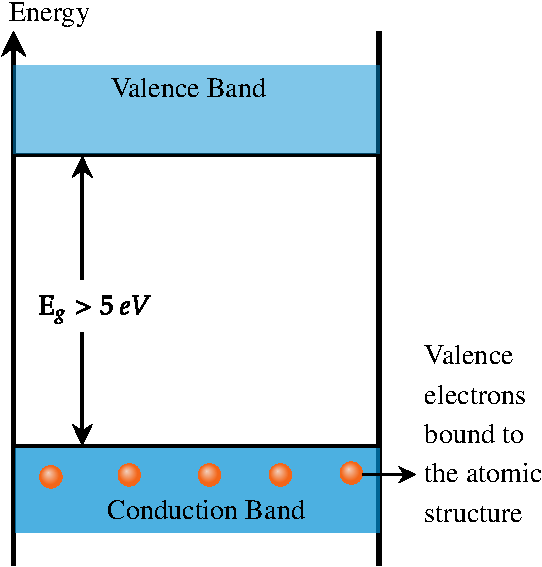
\includegraphics[height=5.5cm,width=5.5cm]{insulatornew}
		\caption{Insulator}
		\label{Insulator}
		\end{figure}
\end{minipage}\hfill
\begin{minipage}{0.30\textwidth}
	\begin{figure}[H]
		\centering
		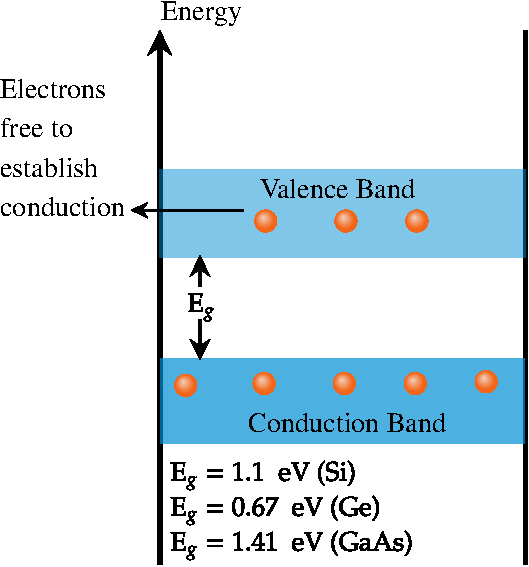
\includegraphics[height=5.5cm,width=5.5cm]{Conductor}
	\caption{Semiconductor}
	\label{Semiconductor}
	\end{figure}
\end{minipage}\hfill
\begin{minipage}{0.30\textwidth}
	\begin{figure}[H]
		\centering
		\includegraphics[height=5.5cm,width=4.1cm]{Semiconductor}
		\caption{Conductor}
		\label{Conductor}
	\end{figure}
\end{minipage}
\section{Semiconductor Materials}
In the section \ref{section-Semiconductors} , it is assumed that there are no external atoms added to the parent semiconductor material. Such semiconductors are referred to as intrinsic semiconductors. Certain impurity atoms when added to the intrinsic semiconductor materials increase their conductivity. Such semiconductors, with added impurity atoms, are called extrinsic semiconductors.
\subsection{Intrinsic Semiconductors}
Intrinsic semiconductors are semiconductors with very low level of impurity concentration. They are essentially as pure as can be available through modern technology. The purity levels are of the order of 1 part in 10 billion. Conduction in intrinsic semiconductors is either due to thermal excitation or due to crystal defects. Silicon and germanium are the two most important semiconductors used. \\
Intrinsic semiconductors can be further classified as direct band gap semiconductors and indirect band gap semiconductors. In a direct band gap semiconductor, the maximum energy of the valence band occurs at the same momentum value as the minimum energy of the conduction band . Thus, in a direct band gap semiconductor, electrons present at the minimum of conduction band combine with holes present at the maximum of valence band while conserving momentum. The energy released due to recombination is emitted in the form of photon of light. Hence, they are used in making light-emitting diodes (LEDs) and laser diodes. 
\begin{example}$\left. \right. $\\
Indirect band gap semiconductors : Gallium arsenide (GaAs) and indium antimonide (InSb)\\
Direct band gap semiconductors : Gallium arsenide and Mercury cadmium telluride.
\end{example}

\subsection{Extrinsic Semiconductors}
The characteristics of semiconductor materials can be altered significantly by the addition of certain impurity atoms into the relatively pure semiconductor material. These impurities, although only added to perhaps 1 part in 10 million, can alter the band structure sufficiently to totally change the electrical properties of the material. A semiconductor material that has been subjected to the doping process is called an extrinsic material. There are two extrinsic materials of immeasurable importance to semiconductor device fabrication: n-type and p-type. Both the n- and p-type materials are formed by adding a predetermined number of impurity atoms into a germanium or silicon base.
\subsection{n-Type Material}
The n-type is created by introducing those impurity elements that have five valence electrons (pentavalent), such as antimony, arsenic, and phosphorus.These impurity atoms are called donor atoms. The effect of this doping process on the relative conductivity can best be described
through the use of the energy-band diagram.
\begin{figure}[H]
	\centering
	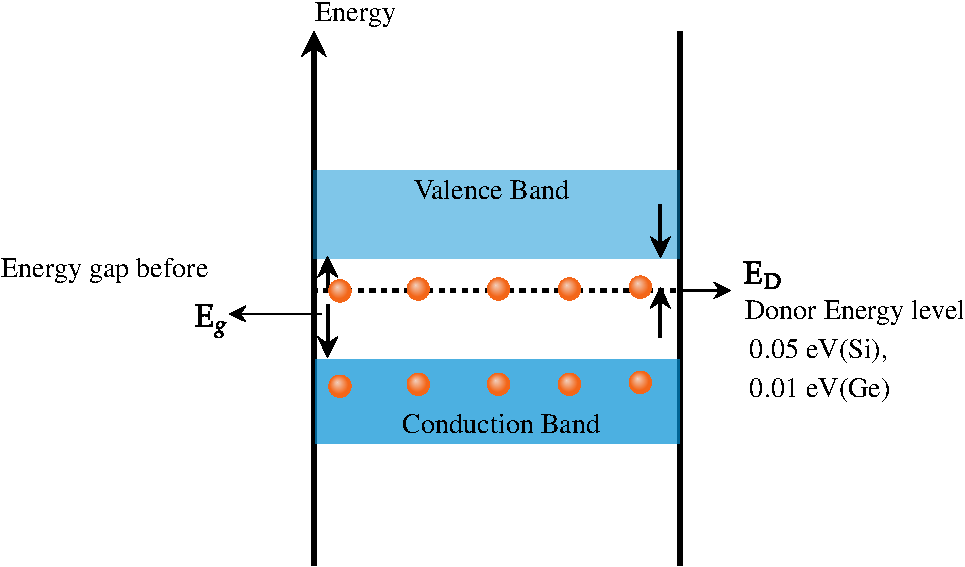
\includegraphics[height=6cm,width=9.8cm]{n type}
	\caption{Energy band diagram of an N-type
		semiconductor.}
	\label{n type}
\end{figure}
The effect of doping creates a discrete energy level called donor energy level in the forbidden band gap with energy level $\left(E_{\mathrm{D}}\right)$ slightly less than the conduction band (Fig. \ref{n type}). The difference between the energy levels of the conduction band and this donor energy level is the energy required to free the electron $(0.01 \mathrm{eV}$ for germanium and $0.05 \mathrm{eV}$ for silicon). At room temperature, almost all the fifth electrons from the donor materials are raised to the conduction band and hence the number of electrons in the conduction band increases significantly.
\subsection{p-Type Material}
A p-type semiconductor is created by adding approximately 1 part in $10^{5}$ parts of trivalent impurity to the intrinsic semiconductor. Trivalent atoms have three electrons in their valence shell and are called acceptor atoms in the context of semiconductor devices. Examples of trivalent impurities include boron (B), indium (In) and gallium (Ga). As there are three electrons in the valence shell of these trivalent impurity atoms, only three covalent bonds can be formed with the neighbouring intrinsic semiconductor atoms and a vacancy exists in the fourth
bond. This vacancy is referred to as the hole and is represented by a small circle. The hole
is ready to accept an electron from a neighbouring atom, thereby creating a hole in the neighbouring atom. This hole in turn is ready to accept an electron thereby creating another hole. In this way, the hole moves through the crystal.
\begin{figure}[H]
	\centering
	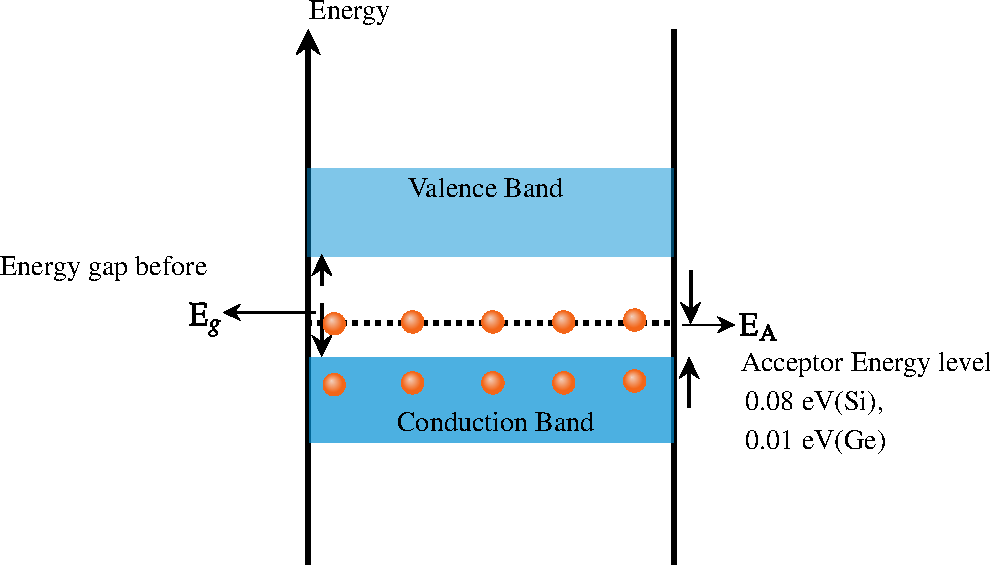
\includegraphics[height=6cm,width=9.8cm]{p type}
	\caption{Energy band diagram of an p-type
		semiconductor.}
	\label{p-type}
\end{figure}
The effect of doping creates a discrete energy level called acceptor level in the forbidden energy band gap with energy level $\left(E_{\mathrm{A}}\right)$ just above the valence band (Fig. \ref{p-type}). The difference between the energy levels of the acceptor band $\left(E_{\mathrm{A}}\right)$ and the valence band $\left(E_{v}\right)$ is the energy required by an electron to leave the valence band and occupy the acceptor band and thereby leaving a hole in the valence band. The difference $\left(E_{\mathrm{A}}-E_{v}\right)$ is of the order of $0.08 \mathrm{eV}$ for silicon and $0.01 \mathrm{eV}$ for germanium.

\subsection{Majority and Minority carriers}
Due to the effect of impurity, $n$-type material has a large number of free electrons whereas $p$-type material has a large number of holes. It may be recalled that even at room temperature, some of the co-valent bonds break, thus releasing an equal number of free electrons and holes. An $n$-type material has its share of electron-hole pairs (released due to breaking of bonds at room temperature) but in addition has a much larger quantity of free electrons due to the effect of impurity. These impurity-caused free electrons are not associated with holes. Consequently, an $n$-type material has a large number of free electrons and a small number of holes. The free electrons in this case are considered majority carriers  since the majority portion of current in $n$-type material is by the flow of free electrons  and the holes are the minority carriers. Similarly, in a $p$-type material, holes outnumber the free electrons as Therefore, holes are the majority carriers and free electrons are the minority carriers.
\subsubsection{ Charge Concentration}
In an intrinsic semiconductor, the number of holes is equal to the number of electrons. Hole and electron pairs are generated by thermal agitation and disappear due to recombination. Therefore, in an intrinsic semiconductor,
\begin{equation}
n=p=n_{\mathrm{i}}
\end{equation}
$n$ = The electron concentration (number of electrons/ $\left.\mathrm{cm}^{3}\right)$\\
$ p$ = The hole concentration (number of holes/cm $/ \mathrm{cm}^{3}$ )\\
$n_{i}$ =The intrinsic concentration.\\
The value of $n_{i}$ is given by the following expression:
\begin{equation}
n_{\mathrm{i}}^{2}=A T^{3} \exp \left(\frac{-E_{\mathrm{g}}}{k T}\right)\label{Charge Concentration}
\end{equation}
or 
\begin{equation}
n_{\mathrm{i}}=AT^{3 / 2} \exp \left(\frac{-E_{g}}{2 k T}  \right)
\end{equation}
Where $T$ is the temperature in kelvin, $E_{\mathrm{g}}$ is the energy gap at $0 \mathrm{~K}, k$ is the Boltzmann constant in $\mathrm{eV} / \mathrm{K}$ and $A$ is the constant.
It is clear from Eq.\ref{Charge Concentration} that the intrinsic concentration $n_{i}$ increases with increase in temperature.
\subsubsection{Electrical Properties}
In a semiconductor, there are two different mechanisms of current flow, namely, the electron flow in the conduction band and the hole flow in the valence band. When an external potential is applied, the free electron may either contribute to the current by drifting through the crystal or combine with a hole in the valence band. The mathematical expression for the current density in any material is as follows:
\begin{equation}
J=\left(n \mu_{\mathrm{n}}+p \mu_{\mathrm{p}}\right) q E
\end{equation}
$J$ = The current density in $\mathrm{A} / \mathrm{cm}^{2} $\\
$n$ = The electron concentration (number of electrons $/ \mathrm{cm}^{3}$ )\\ $p$ = The hole concentration (number of holes/cm³)\\ $\mu_{\mathrm{n}}$ = The mobility of an electron in the material in $\mathrm{cm}^{2} / \mathrm{V} \cdot \mathrm{s}$\\ $ \mu_{\mathrm{p}}$ =  The mobility of a hole in the material in $\mathrm{cm}^{2} / \mathrm{V} \cdot \mathrm{s}$\\ $q$= The charge of an electron $=1.6 \times 10^{-19} \mathrm{C}$ \\$E$ = The applied electric field in $\mathrm{V} / \mathrm{cm}$.\\
This current is due to the potential gradient created by the applied electric field and is referred to as $d r i f t$ current density. The expression for conductivity $(\sigma)$ is as follows:
\begin{align}
\sigma&=\left(n \mu_{\mathrm{n}}+p \mu_{\mathrm{p}}\right) q\\
\text{As in an intrinsic }&\text{semiconductor, $n=p=n_{\mathrm{i}}$} \\
\because J&=\left(\mu_{\mathrm{n}}+\mu_{\mathrm{p}}\right) n_{\mathrm{i}} q E  \\
\text{And }, \sigma&=\left(\mu_{\mathrm{n}}+\mu_{\mathrm{p}}\right) n_{\mathrm{i}} q
\end{align}
\subsubsection{Fermi Level}
The probability that an energy level in a semiconductor is occupied by an electron is given by the following expression:
\begin{equation}
f(E)=\frac{1}{1+\exp \left[\left(E-E_{f}\right) / k T\right]}
\end{equation}
Where $f(E)$ is the Fermi-Dirac probability function = Probability of finding an electron in the energy state $E, k$ is the Boltzmann constant $=8.642 \times 10^{-5} \mathrm{eV} / \mathrm{K}, T$ is the temperature in kelvin and $E_{f}$ is the Fermi level in eV.\\
The Fermi level remains at the centre of the forbidden band gap and is given by,
\begin{equation}
E_{f}=\frac{E_{c}+E_{v}}{2}
\end{equation}
Where $E_{c}$ is the energy of the conduction band and $E_{v}$ is the energy of the valence band.
\begin{enumerate}
	\item \textbf{Fermi level of n-type semiconductors }\\\\
	\textbf{At low temperature}\\
	\begin{align*}
	\frac{E_{f}}{k_{B} T}&=\frac{E_{c}+E_{d}}{2 k_{B} T}+(1 / 2) \ln \left[\frac{N_{d}}{N_{c}}\right]\\
	\text{Where }\ N_d&= \text{density of donor atoms}.\\
	N_c&=2\left[ (2\pi m_e^* k_BT)/h^2\right] ^{3/2}\\
	E_f&=\frac{E_{c}+E_{d}}{2}+(1 / 2) \ln \left[\frac{N_{d}}{N_{c}}\right]\\
	\text{At $T=0 $ } E_f&=\frac{E_c+E_d}{2}
	\end{align*}
	i.e. Fermi level lies exactly half way between the donor level and bottom of the conduction band. As $T$ increases, Fermi level drops. Also for a given temperature, the Fermi level shifts upward as the concentration increases.\\
	\textbf{At high temperature}\\
	\begin{align*}
	E_{f}&=E_{c}+k_{B} T \ln \frac{N_{d}}{N_{c}}\\&=E_{c}-k_{B} T \ln \frac{N_{c}}{N_{d}}
	\end{align*}
	
	From this equation we can say that $E_f$ drops as $T$ increases.$E_f\rightarrow E_g/2$ if $k_BT>>(E_c-E_d)$All this meansis that intrinsic carriers,which are produced in equal concentration of holes aand electrons eventuaally swamps the impurirties and make the material essentially intrinsic again if the temperature is high enough.
	\item \textbf{Fermi level of p-type semiconductors}\\
	\textbf{At low temperature}\\
	\begin{align*}
	E_f&=\frac{E_{a}+E_{v}}{2}+\left[\frac{k_{B} T}{2}\right] \ln \frac{N_{v}}{N_{a}}\\
	\text{Where } N_a&= \text{Density of acceptor atom}\\
   N_v&=2\left[ (2\pi m_p^* k_BT)/h^2\right] ^{3/2}\\
	\text{At $T=0$, } E_{f}&=\left(E_{a}+E_{v}\right) / 2
	\end{align*}
	i.e. Fermi level lies exactly half way between the acceptor level and top of the valence band. As $T$ increases, Fermi level shifts upward. Also for a given temperature the Fermi level shifts. downward as the concentration increases.\\
	\textbf{At high temperature} \\
	$$E_{f}=E_{v}+k_{B} T \ln \frac{N_{v}}{N_{a}}$$
	From this equation we can say that $E_f$ moves upwards as T increases.$E_f\rightarrow E_g/2$ if $ k_BT>>(E_a-E_v)$. All this means that intrinsic carriers which are produced in equal concentration of holes and electrons , eventually swamps the impurities and make the material essentially intrinsic again if the temperature is high enough.
\end{enumerate}

\begin{exercise}
	Calculate the mobility of the electrons in copper obeying classical laws. Given that the density of copper $=8.92 \times 10^{3} \mathrm{~kg} / \mathrm{m}^{3}$, Resistivity of copper $=1.73 \times 10^{-8}$ ohm-m, atomic weight of copper $=63.5$ and Avogadro's number $=6.02 \times 10^{26}$ per k-mol.
\end{exercise}
\begin{answer}
	Number of free electrons per $\mathrm{m}^{3}, n=\frac{\text { No. of free electrons per atom } \times N_{\mathrm{A}} \times D}{\text { Atomic weight }}$
	$$
	\begin{aligned}
	&\qquad n=\frac{1 \times 6.02 \times 10^{26} \times 8.92 \times 10^{3}}{63.5} \text { per } \mathrm{m}^{3}=8.456 \times 10^{28} \text { per } \mathrm{m}^{3} \\
	&\qquad \begin{aligned}
	\rho &=\frac{1}{n e \mu} \quad \text { where } \mu=\text { mobility } \\
	\mu &=\frac{1}{n e \rho}=\frac{1}{8.456 \times 10^{28} \times 1.6 \times 10^{-9} \times 1.73 \times 10^{-8}} \\
	&=0.0427 \mathrm{~m}^{2} / \mathrm{V}_{\mathrm{s}}
	\end{aligned}
	\end{aligned}
	$$
\end{answer}
\newpage
\begin{abox}
	Semiconductor Diodes
\end{abox}
\section{P-N Junction}
A semiconductor diode is a polarity sensitive two terminal device comprising a p-n junction formed ( The regions p and n are united by a metallurgical connection. ) between a p-type semiconductor material and an n-type semiconductor material. In an n-type semiconductor, electrons are the majority carriers and holes are the minority carriers, whereas in a p-type semiconductor, holes are the majority carriers and electrons are the minority carriers. A p-n junction is formed by introducing the donor impurities on one side and acceptor impurities on the other side of a single crystal of a semiconductor. Figure.\ref{Diode} shows the circuit symbol of a p-n junction diode.\\
\begin{minipage}{0.35\textwidth}
\begin{figure}[H]
	\centering
	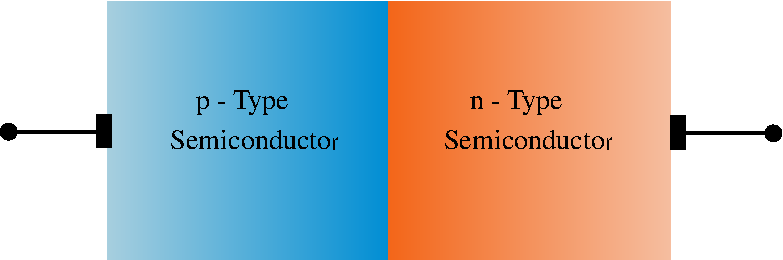
\includegraphics[height=2.8cm,width=7.8cm]{pn junction new}
	\caption{p-n Junction.}
	\label{}
\end{figure}
\end{minipage}\hfil
\begin{minipage}{0.55\textwidth}
	\begin{figure}[H]
		\centering
		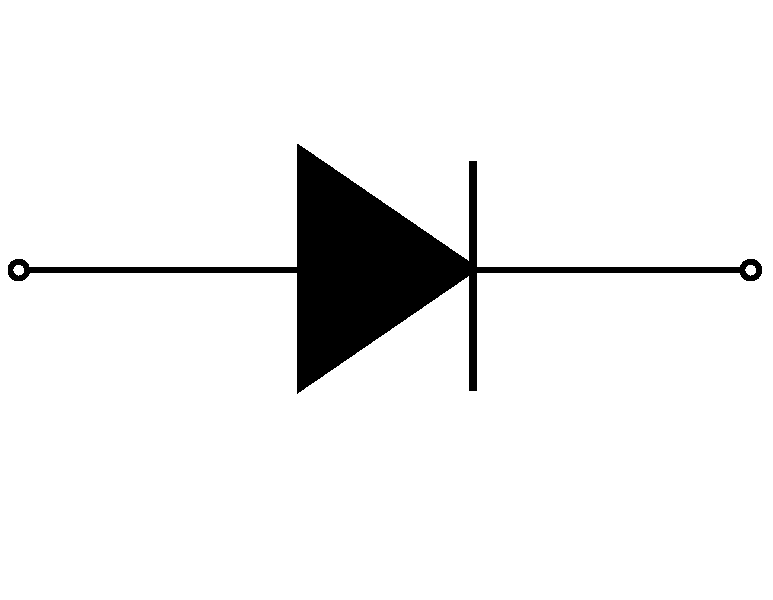
\includegraphics[height=2.8cm,width=4cm]{diagram-20220617(4)}
		\caption{Schematic digram of p-n junction diode.}
		\label{Diode}
	\end{figure}
\end{minipage}\\\\
The electrons in the n region and holes in the p region combine near the junction, resulting in a region near the junction that is devoid of free electrons and holes. This region of uncovered positive and negative ions is called the depletion region due to depletion of free carriers in
this region. The thickness of this region is of the order of 0.5 $ \mathrm{\mu m}$
\subsubsection{Majority carrier flow}
Electrons (majority carriers) in the n region and negatively charged ions in the p region, near the junction repel each other. Similarly, holes in the p region (majority carriers) and positively charged ions in the n region, near the junction also repel each other. An effective potential of the order of few tenths of a volt, referred to as the contact potential or the barrier potential, is developed across the depletion region. However, some of these holes and electrons have sufficient kinetic energy to overcome the contact potential and be able to
pass through the depletion region. This results in a flow of electrons from the n region to the p region and flow of holes from the p region to the n region. This constitutes the majority carrier flow .
\subsubsection{Minority carrier flow}
Holes (minority carriers) that are present in the depletion region of the n region will pass to the p region. Similarly, electrons (minority carriers) that are present in the depletion region of the p region will pass to the n region. This constitutes the minority carrier flow.\\\\
Since the diode is a two-terminal device, the application of a voltage across its terminals leaves three possibilities: no bias $\left(V_{D}=0 \mathrm{~V}\right)$, forward bias $\left(V_{D}>0 \mathrm{~V}\right)$, and reverse bias $\left(V_{D}<0 \mathrm{~V}\right)$. Each is a condition that will result in a response that the user must clearly understand if the device is to be applied effectively.
\subsection{No bias $\left(V_{D}=0 \mathrm{~V}\right)$}
The relative magnitudes of the minority and the majority flow vectors are such that the net flow in either direction is zero. This is referred to as the open circuit condition of the semiconductor diode where no bias ­voltage is applied to the diode. In other words, in the absence of an applied bias voltage, the net flow of ­current in a semiconductor diode is zero.
\begin{figure}[H]
	\centering
	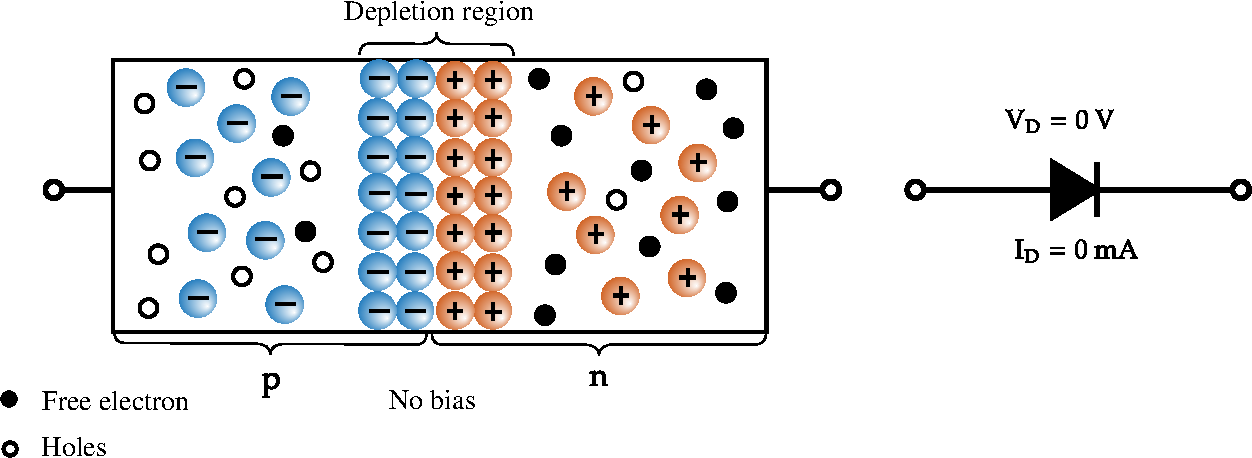
\includegraphics[height=5cm,width=13.5cm]{pn junction}
	\caption{p-n junction with
		no external bias.}
	\label{No bias}
\end{figure}
\subsection{Reverse Bias $\left(V_{D}<0 \mathrm{~V}\right)$}
If an external potential of $V$ volts is applied across the $p-n$ junction such that the positive terminal is connected to the $n$-type material and the negative terminal is connected to the $p$-type material as shown in Fig. $1.16$, the number of uncovered positive ions in the depletion region of the $n$-type material will increase due to the large number of "free" electrons drawn to the positive potential of the applied voltage. For similar reasons, the number of uncovered negative ions will increase in the $p$-type material. The net effect, therefore, is a widening of the depletion region. This widening of the depletion region will establish too great a barrier for the majority carriers to overcome, effectively reducing the majority carrier flow to zero as shown in Fig.\ref{Reverse bias}. The number of minority carriers, however, that find themselves entering the depletion region will not change, resulting in minority carrier flow vectors of the same magnitude indicated in Fig. \ref{No bias} with no applied voltage.
The current that exists under reverse bias conditions is called the reverse saturation current and is represented by $\mathrm{I_s}$ .
\begin{figure}[H]
	\centering
	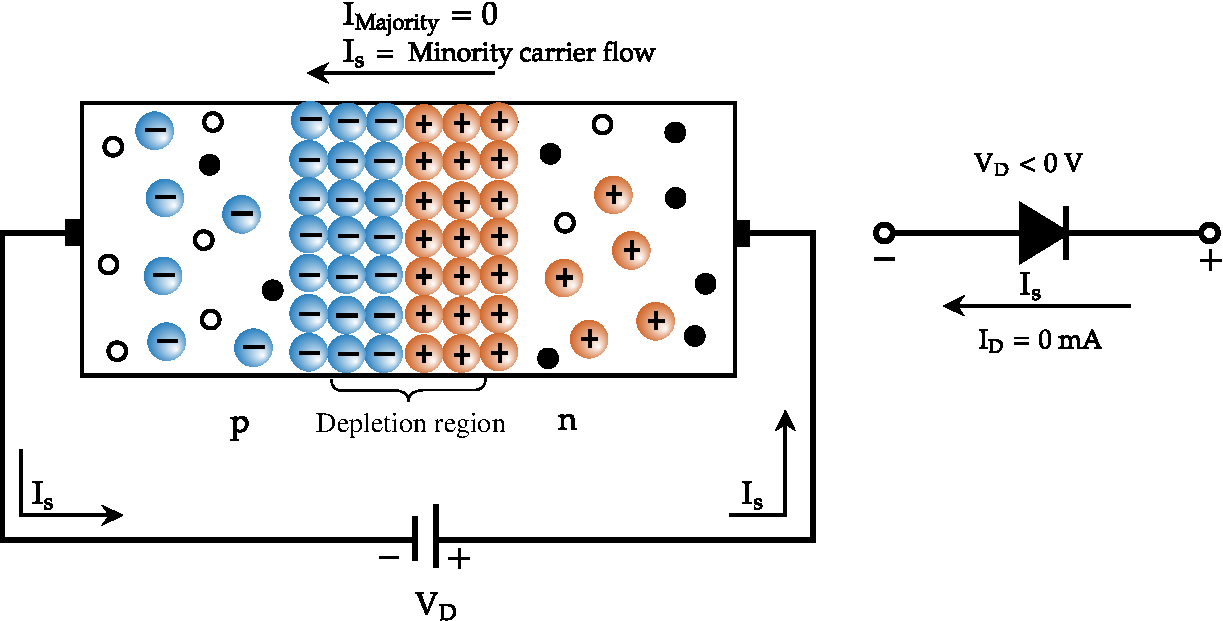
\includegraphics[height=6cm,width=11.5cm]{Reverse bias}
	\caption{Reverse bias}
	\label{Reverse bias}
\end{figure}
The reverse saturation current is seldom more than a few microamperes except for high-power devices.
\subsection{Forward-Bias  $\left(V_{D}>0 \mathrm{~V}\right)$}
A forward-bias or “on” condition is established by applying the positive potential to the p-type material and the negative potential to the n-type material as shown in Fig. \ref{Forward Bias}. The application of a forward-bias potential $\mathrm{V_D}$ will “pressure” electrons in the n-type material and holes in the p-type material to recombine with the ions near the boundary and reduce the width of the depletion region. An electron of the n type material sees a reduced barrier at the junction due to the reduced depletion region and a strong attraction for the positive potential applied to the p-type material.As the applied bias increases in magnitude,the depletion layer will continue decrease in width untill a flood of electron can pass through the junction,resulting in a exponential rise in the current as shown in the forward bias region of the characterestics curve.
\begin{figure}[H]
	\centering
	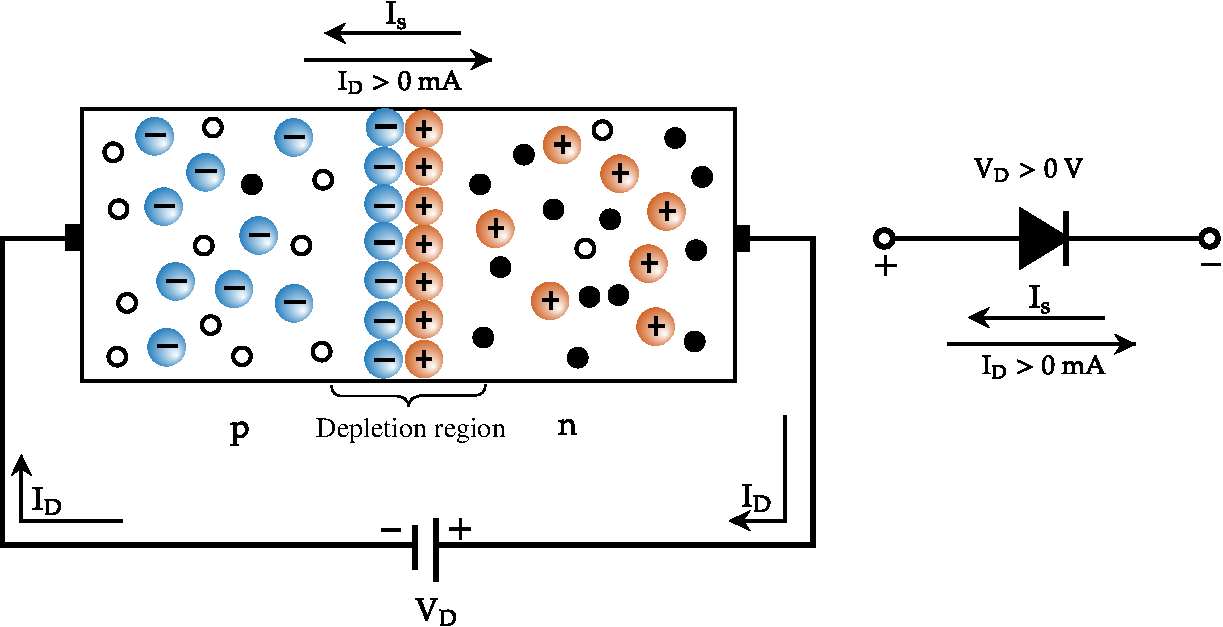
\includegraphics[height=6cm,width=11.5cm]{Foreward Bias}
	\caption{Forward Bias}
	\label{Forward Bias}
\end{figure}
\subsection{V-I Characteristics}
Volt-ampere or $V$-I characteristic of a pn junction is the curve between voltage across the junction and the circuit current. Usually, voltage is taken along $x$ axis and current along $y$-axis. The characteristics can be studied under three heads, namely; zero external voltage, forward bias and reverse bias.
\begin{figure}[H]
	\centering
	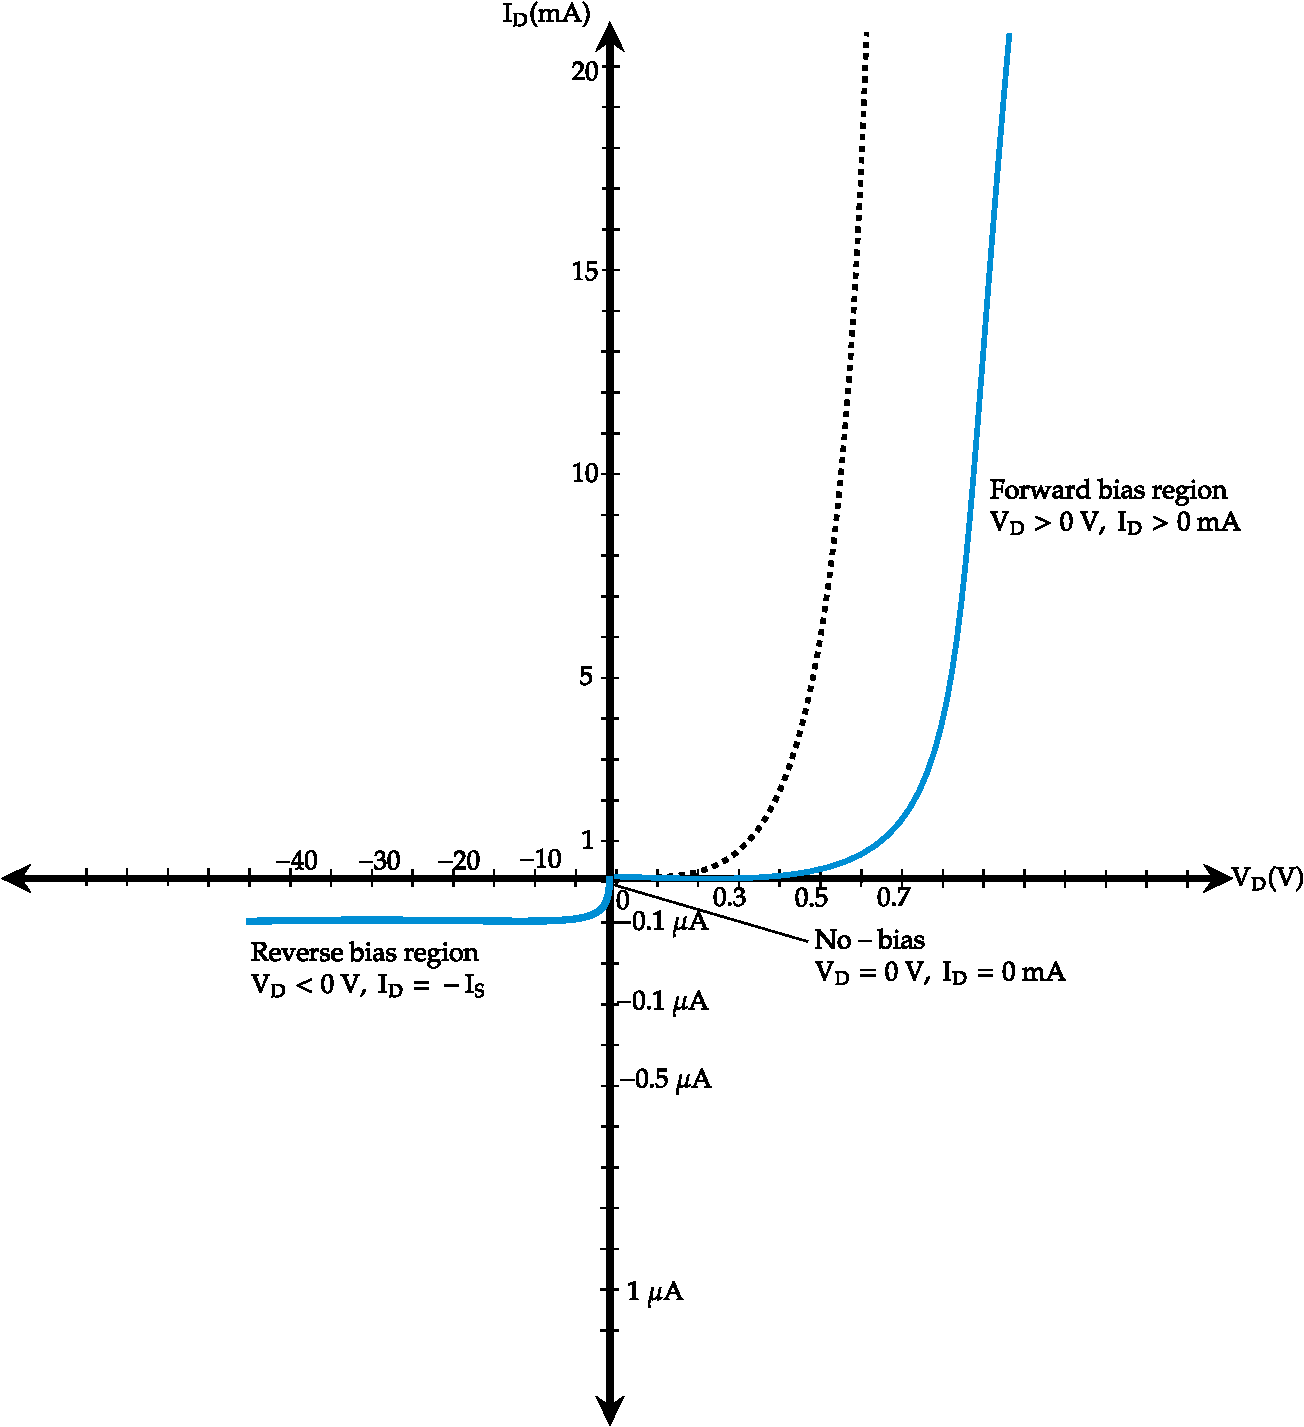
\includegraphics[height=11cm,width=10cm]{V-I charecteristics si}
	\caption{V-I charesterics of Silicon}
	\label{V-I characterics of Silicon}
\end{figure}
\subsubsection{No bias}
 When the external voltage is zeo, the circuit is open and the potential barrier does not permit current flow. Then the circuit current is zero.
\subsubsection{Forward bias}
 With forward bias to the $p n$ junction , the potential barrier is reduced. At some forward voltage $(0.7 \mathrm{~V}$ for $\mathrm{Si}$ and $0.3 \mathrm{~V}$ for Ge), the potential barrier is altogether eliminated and current starts flowing in the circuit. From now onwards, the current increases with the increase in forward voltage. Thus, a rising curve  is obtained with forward bias as shown in Fig.\ref{V-I characterics of Silicon}. From the forward characteristic, it is seen that at first , the current increases very slowly and the curve is non-linear. It is because the external applied voltage is used up in overcoming the potential barrier. However, once the external voltage exceeds the potential barrier voltage, the $p n$ junction behaves like an ordinary conductor. Therefore, the current rises very sharply with increase in external voltage . The curve is almost linear.
\subsubsection{Reverse bias}
 With reverse bias to the $p - n$ junction potential barrier at the junction is increased. Therefore, the junction resistance becomes very high and practically no current flows through the circuit. However, in practice, a very small current (of the order of $\mu A$ ) flows in the circuit with reverse bias as shown in the reverse characteristics, this is called as reverse saturation current, $I_{s}$ and is due to minority carriers. 
 If reverse voltage is increased continuously, the kinetic energy of electrons (minority carriers) may become high enough to knock out electrons from the semiconductor atoms. At this stage break down of the junction occurs, characterised by a sudden rise of reverse current and a sudden fall of the resistance of barrier region. This may destroy the junction permanently.
\begin{center}
	\framebox{
		\parbox[t][5cm]{15cm}{
			
			\addvspace{0.2cm} 
			
		\textbf{Break down Voltage:} It is the minimum reverse voltage at which $p- n$ junction breaks down with sudden rise in reverse current.Under normal reverse voltage, a very little reverse current flows through a pn junction. However, if the reverse voltage attains a high value, the junction may break down with sudden rise in reverse current.\\\\
	\textbf{Knee voltage:} It is the forward voltage at which the current through the junction starts to increase rapidly. When a diode is forward biased, it conducts current very slowly until we overcome the potential barrier. Once the applied forward voltage exceeds the knee voltage, the current starts increasing rapidly. It may be added here that in order to get useful current through a pn junction, the applied voltage must be more than the knee voltage.} }
\end{center}
\begin{note}
	The forward current through a pn junction is due to the majority carriers produced by the impurity. However, reverse current is due to the minority carriers produced due to breaking of some co-valent bonds at room temperature.
\end{note}
\subsection{Limitations in the operating conditions}
Every $p n$ junction has limiting values of maximum forward current, peak inverse voltage and maximum power rating. The $p n$ junction will give satisfactory performance if it is operated within these limiting values. However, if these values are exceeded, the $p n$ junction may be destroyed due to excessive heat.
\begin{enumerate}
	\item \textbf{ Maximum forward current:} It is the highest instantaneous forward current that a $p-n$ junction can conduct without damage to the junction. Manufacturer's data sheet usually specifies this rating. If the forward current in a $p-n$ junction is more than this rating, the junction will be destroyed due to overheating.
	\item \textbf{Peak inverse voltage (PIV):} It is the maximum reverse voltage that can be applied to the $p-n$ junction without damage to the junction. If the reverse voltage across the junction exceeds its PIV, the junction may be destroyed due to excessive heat. The peak inverse voltage is of particular importance in rectifier service. A pn junction i.e. a crystal diode is used as a rectifier to change alternating current into direct current. In such applications, care should be taken that reverse voltage across the diode during negative half-cycle of a.c. does not exceed the PIV of diode.
	\item \textbf{Maximum power rating:} It is the maximum power that can be dissipated at the junction without damaging it. The power dissipated at the junction is equal to the product of junction current and the voltage across the junction. 
\end{enumerate}
\subsection{Diode equation}
It can be demonstated through the use of solid state physics that the general characterestics of a semiconductor diode can be defined by the following equation reffered to as Shockley equation,\textbf{for the forward and reverse bias regions,}
\begin{equation}
I_{D}=I_{s}\left(e^{k V_{D} / T_{K}}-1\right)
\end{equation}
\begin{align*}
I_S& =\text{The reverse saturation current }\\
V_D &=\text{The applied forward voltage across the diode}\\
k&=11,600 / \eta \text{with $\eta=1$ for Ge and $\eta=2$ for Si for relatively low levels of diode current }\\& \left. \right. \hspace{0.3cm} \text{(at or below the knee of the curve) and $\eta=1$ for Ge and Si for higher levels of diode }\\& \left. \right. \hspace{0.3cm} \text{ current (in the rapidly increasing section of the curve)}\\
T_K&=\text{ The absolute temperature in kelvin}\\
T_{K}&=T_{C}+273^{\circ}\\
V_{T} &=\frac{k T_{K}}{q} \ (\text{Thermal Voltage})
\end{align*}
Thus current can flow readly in one direction through a p-n junction but hardly at all in the other direction ,which makes such a junction as ideal rectifier in the electric circuit. The greater the applied voltage the greater the current in the forward direction.
\begin{exercise}
At a temperature of $27^{\circ} \mathrm{C}$ (common temperature for components in an enclosed operating system), determine the thermal voltage $V_{T}$.
\end{exercise}
\begin{answer}
$$
\begin{aligned}
T &=273+{ }^{\circ} \mathrm{C}=273+27=300 \mathrm{~K} \\
V_{T} &=\frac{k T_{K}}{q}=\frac{\left(1.38 \times 10^{-23} \mathrm{~J} / \mathrm{K}\right)(30 \mathrm{~K})}{1.6 \times 10^{-19} \mathrm{C}} \\
&=25.875 \mathrm{mV} \cong 26 \mathrm{mV}
\end{aligned}
$$
The thermal voltage will become an important parameter in the analysis to follow in this chapter and a number of those to follow.
\end{answer}  
\section{Ideal Diode Versus Practical Diode}
\begin{figure}[H]
\centering
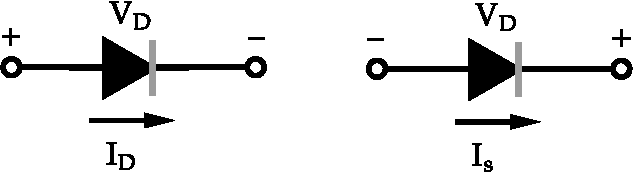
\includegraphics[height=2cm,width=7cm]{fb n rb}
\caption{Forward bias and  Reverse bias}
\label{fb n rb}
\end{figure}
We found that a p-n junction will permit generous flow of charge when forward biased and a very small level of current when reverse biased. Both conditions are viewed in the figure \ref{fb n rb}.\\ \textit{The semiconductoe diode behaves in a manner similar to a mechanical switch in that it can control whether current flow between it's two terminals.}\\
Ideally if the semiconductor diode is to behave like a closed switch in the forward bias region ,the resisstance of the diode should be $ 0\Omega$. In the reverse bias region its resistance should be $ \infty\Omega$ to represents the open circuit equivalent.

\section{Resistance levels}
As the operating point of the diode moves from one region to another the resistance of the diode will also change due to the non linear shape of the charactrestics curve. The type of applied voltage or signal will define the resistance level of interest.
\begin{enumerate}
\item \textbf{DC or static resistance}\\
The application of a dc voltage to a circuit containing a semiconductor diode will result in an operating point on the characteristic curve that will not change with time. The resistance of the diode at the operating point can be found simply by finding the corresponding levels of $V_{D}$ and $I_{D}$ and applying the following equation:
\begin{equation}
R_{D}=\frac{V_{D}}{I_{D}}
\end{equation}
The dc resistance levels at the knee and below will be greater than the resistance levels obtained for the vertical rise section of the characteristics. The resistance levels in the reverse-bias region will naturally be quite high.
\item \textbf{AC or dynamic resistance}\\
The dc resistance of a diode is independent of the shape of the characteristic in the region surrounding the point of interest.
If a sinusoidal rather than a dc input is applied, the situation will change completely. The varying input will move the instantaneous operating point up and down a region of the characteristics and thus defines a specific change in current and voltage , with no applied varying signal, the point of operation would be the $Q$-point appearing will be determined by the applied dc levels. The designation $Q$-point is derived from the word quiescent, which means "still or unvarying."
\begin{figure}[H]
	\centering
	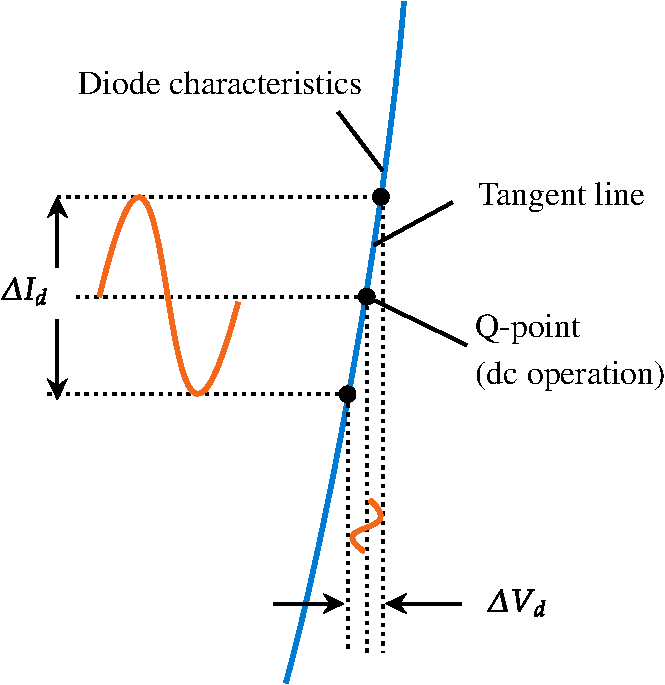
\includegraphics[height=6cm,width=7cm]{ac resistance}
	\caption{AC or dynamic resistance}
	\label{ac resistance}
\end{figure}
A straight line drawn tangent to the curve through the $Q$-point as shown in figure. \ref{ac resistance} will define a particular change in voltage and current that can be used to determine the $a c$ or dynamic resistance for this region of the diode characteristics. An effort should be made to keep the change in voltage and current as small as possible and equidistant to either side of the $Q$-point. In equation form,
\begin{equation}
r_{d}=\frac{\Delta V_{d}}{\Delta I_{d}}
\end{equation}
Where $\Delta$ signifies a finite change in the quantity. The steeper the slope, the lower is the value of $\Delta V_{d}$ for the same change in $\Delta I_{d}$ and the lower is the resistance. The ac resistance in the vertical-rise region of the characteristic is therefore quite small, whereas the ac resistance is much higher at low current levels.
In general, therefore, the lower the $Q$-point of operation (smaller current or lower voltage), the higher is the ac resistance.\\
We have found the dynamic resistance graphically, but there is a basic definition in differential calculus that states:
The derivative of a function at a point is equal to the slope of the tangent line drawn
at that point.
\begin{align*}
\frac{d}{d V_{D}}\left(I_{D}\right)&=\frac{d}{d V}\left[I_{S}\left(e^{k V_{D} / T_{K}}-1\right)\right]\\
\text{And } \ \frac{d I_{D}}{d V_{D}}&=\frac{k}{T_{K}}\left(I_{D}+I_{s}\right)
\intertext{After we apply differential calculus. In general, $I_{D} \gg I_{s}$ in the vertical-slope section of the characteristics ,}
\frac{d I_{D}}{d V_{D}} &\cong \frac{k}{T_{K}} I_{D}
\intertext{Flipping the result to define a resistance ratio $(R=V / I)$ gives,}
\frac{d V_{D}}{d I_{D}}&=r_{d}=\frac{ T_{K}}{kI_{D}}
\end{align*}
\item \textbf{Average AC resistance}
If the input signal is sufficiently large to produce a broad swing the resistance associated with the device for this region is called average AC resistance.The average AC resistance is by definition the resistance determined by a straight line drawn between the two intersections established by the maxima and minimum values of input voltage.In equation form 
$$r_{av}=\frac{\Delta V_d}{\Delta I_d}|_{pt.to.pt}$$
\end{enumerate}
\section{Capacitance in P-N junction diode}
\begin{itemize}
\item  The P and N regions are essentially low resistance areas due to high concentration of majority carriers.
\item - The depletion region, which is depleted of charge carriers, serves as an effective insulation.
\item  Hence, a diode has a very high resistance depletion region (Insulator) sandwiched between low resistive P and N regions
\item  The $P$ and $N$ regions acts as plates of capacitor, while the depletion region acts as the insulating dielectric
\item  Thus a P-N junction diode can be compared to a charged capacitor and the capacitances associated with the P-N junction are:\\
(i) Transition capacitance,\\
(ii) Diffusion capacitance
\end{itemize}
\paragraph{Transition capacitance}  
\begin{itemize}
\item  This is the capacitance of a reverse biased diode.
\item  It is also known as Space-charge capacitance or junction capacitance
\item $$\begin{aligned}
&\qquad C_{T} \text { is given by } C_{T}=\frac{\varepsilon A}{W} \\
&\text { Where } \varepsilon=\text { the permittivity of semiconductor material } \\
&\qquad 
\begin{aligned}
A &=\text { Cross-sectional area of junction } \\
W &=\text { width of depletion region }
\end{aligned}
\end{aligned}$$
\item  The $C_{T}$ can be controlled by varying the width of depletion region $(W)$. The $W$ can be varied with the applied reverse bias voltage.
\item As the reverse bias voltage increases, the $W$ increases and hence $C_{T}$ decreases and viceversa.
\end{itemize}
\paragraph{Varactor Diodes or Vari-caps:}
\begin{itemize}
\item The Si diodes designed for getting variable capacitance effects under reverse bias are called ${\text { Varactor diodes. }}$ They are also called voltage variable capacitance diodes.
\item  The ty pical variation in capacitance that can be obtained is 2-12 $\mu F$ and 20-28 $\mu F$.
\end{itemize}
\paragraph{Diffussion capacitance $C_D$}
\begin{itemize}
\item This is the capacitance of a forward biased diode.
\item During forward bias, the barrier width of the diode decreases.
\item $C_{D}$ is given by $C_{D}=\frac{\tau I}{\eta V_{T}}$
Where $\tau=$ mean life time the charge carrier
$I=$ forward current through the diode $($ Amp $)$
$\eta=\left\{\begin{array}{l}1 ; \text { for } G e \\ 2 ; \text { for } S i\end{array}\right.$
$V_{T}=$ Volt equivalent of temperature (Volts) $=\frac{T}{11,600}$ Volts, T in Kelvin
At room temperature $\left(27^{0} \mathrm{C}=300 \mathrm{~K}\right), V_{T}=300 / 11,600=0.025862 \mathrm{~V} \approx 26 \mathrm{mV}$
\item  $C_{D}$ of a forward biased diode $\propto$ Diode forward current $(I)$
\item  $C_{D}$ ranges from 10 to $1000 \mathrm{pF}$
\item $C_{D}$ of a forward biased diode $>>C_{T}$ of a reverse biased diode
\end{itemize}
\section{Zener diode}
There is a point where the application of too negative a voltage will result in a sharp change in the characteristics, as shown in Fig. 1.22. The current increases at a very rapid rate
in a direction opposite to that of the positive voltage region. The reverse bias potential that results in this dramatic change in characteristics is called the Zener potential
and is given the symbol $V_ Z $.
\begin{figure}[H]
\centering
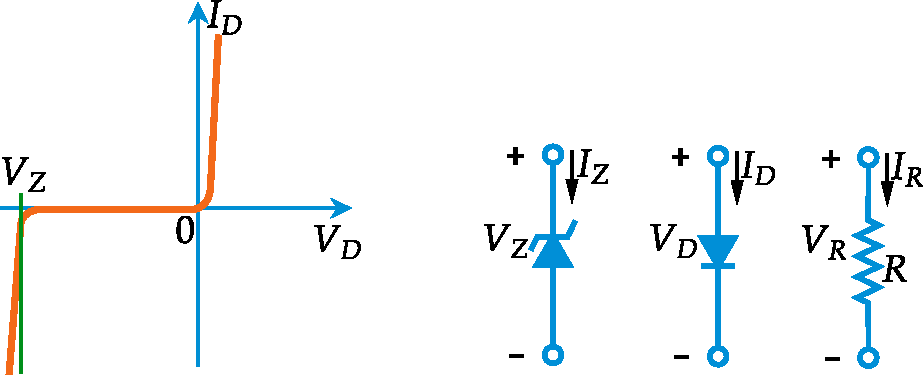
\includegraphics[height=4cm,width=10cm]{zener}
\caption{}
\label{}
\end{figure}
\par As the voltage across the diode increases in the reverse-bias region, the velocity of the minority carriers responsible for the reverse saturation current $I_{s}$ will also increase. Eventually, their velocity and associated kinetic energy $\left(W_{K}=\frac{1}{2} m v^{2}\right)$ will be sufficient to release additional carriers through collisions with otherwise stable atomic structures. That is, an ionization process will result whereby valence electrons absorb sufficient energy to leave the parent atom. These additional carriers can then aid the ionization process to the point where a high avalanche current is established and the avalanche breakdown region determined.\\
The break down voltage can be reduced (up to -1.8 voltage in some diodes) by increasing the doping level of p and n type material is called Zener breakdown and it will contribute a the sharp changes in the characteristic. It occurs because there is a strong electric field in the region of the junction that can disrupt the bonding forces within the atom and "generate" carriers. Although the Zener breakdown mechanism is a significant contributor only at lower levels of $V_{B V}$, this sharp change in the characteristic at any level is called the Zener region, and diodes employing this unique portion of the characteristic of a  $p-n$ junction are called Zener diodes.\\
 The breakdown region of the semiconductor diode described must be avoided if the response of a system is not to be completely altered by the sharp change in characteristics in this reverse-voltage region\\
 \textit{The maximum reverse bias potential that can be applied before entering the breakdown region is called peak inverse voltage(reffered to simply as PIV rating) or the peak reverse voltage(denoted as PRV rating)}
\subsection{Zener diode as a voltage regulator}
\par A zener diode can be used as a voltage regulator to provide a constant voltage from a source whose voltage may vary over sufficient range. The circuit arrangement is shown in Figure.\ref{Zener as regulator} .The zener diode of zener voltage $V_{Z}$ is reverse connected across the load $R_{L}$ across which constant output is desired. The series resistance $R$ absorbs the output voltage fluctuations so as to maintain constant voltage across the load. It may be noted that the zener will maintain a constant voltage $V_{Z}\left(=E_{0}\right)$ across the load so long as the input voltage does not fall below $V_{Z}$.\\
 Now we can discuss how a zener diode regulate voltage across a circuit if the input voltage$(E_0)$ and load resistance $(R_L)$changes.
\begin{figure}[H]
\centering
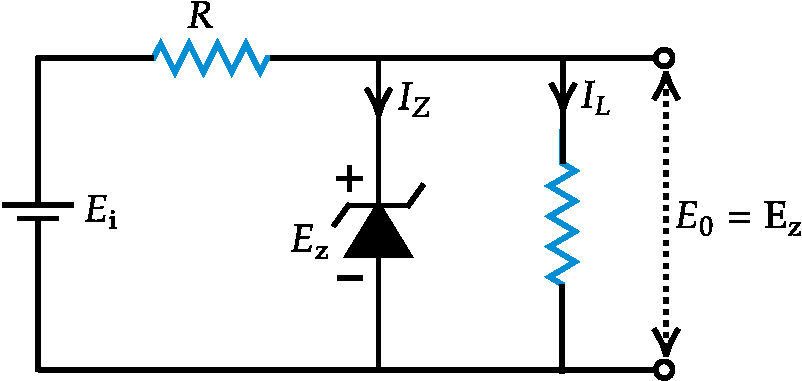
\includegraphics[height=3.5cm,width=7cm]{diagram-20211104(4)-crop}
\caption{Zener diode as a voltage regulator}
\label{Zener as regulator}
\end{figure}
\begin{itemize}
\item \textbf{When the input voltage increases:}\
Since the zener is in the breakdown region, the zener diode is equivalent to a battery with voltage $V z$ . It is clear that output voltage remains constant at $V_{Z}\left(=E_{0}\right)$. The excess voltage is dropped across the series resistance $R$. This will cause an increase in the value of total current $I(I=I_Z+I_L)$. The zener will conduct the increase of current in $I$ while the load current remains constant. Hence, output voltage $E_{0}$ remains constant irrespective of the changes in the input voltage $E_{i}$.
\item \textbf{When the load resistance decreases:}\
Now suppose that input voltage is constant but the load resistance $R_{L}$ decreases. This will cause an increase in load current. The extra current can not come from the source because drop in $R$  will not change because the zener is within its regulating range. The additional load current will come from a decrease in zener current $I_{Z}$. Consequently, the output voltage stays at constant value.\\
Voltage drop across $R$
$$V=E_{i}-E_{o}$$
Current through $R$ $$I=I_{Z}+I_{L}$$
Applying ohm's law, we have,
$$
R=\frac{E_{i}-E_{o}}{l_{Z}+I_{L}}
$$
\item \textbf{Maximum and minimum value of R}\\
$\mathbf{(1)}$ The minimum value s of R that prevents the diode from being damaged is given by \\
$$R_{min}=\frac{E_{i,max}-E_{z}}{I_{Z_{max}}}$$
Where $I_{Z_{max}}$ can be obtained from $P_{Z_{max}}=E_{Z}.I_{Z_{max}}$\\
$P_{Z_{max}}$ is normally specified by the manufacturer which is the maximum power that the zener diode can tolerate.\\
$\mathbf{(2)}$ The maximum permitted value of R is set by the condition that current through the zener diode must not go below $I_{ZK}$ (Which is the knee current that corresponds to the knee of reverse characterestics curve)
$$R_{max}=\frac{E_{i,min}-E_{z}}{I_{L,max}+I_{ZK}}=\frac{E_{i,min}-E_{z}}{I_{L,max}}$$
\end{itemize}
\begin{exercise}
The circuit shown in the figure,find:
\begin{figure}[H]
	\centering
	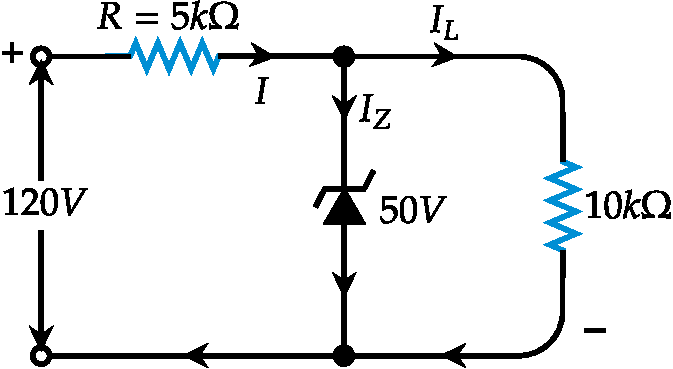
\includegraphics[height=3cm,width=6cm]{zener 1}
	\caption{}
	\label{}
\end{figure}
\begin{enumerate}
	\item  The output voltage
	\item The voltage drop across the series resistance
	\item The current through the zener diode
\end{enumerate}

\end{exercise}
\begin{answer}
If you remove the zener diode the  voltage across the load resistance is given by
$$V=\frac{R_L}{R_L+R}\times E_i$$
$$V=\frac{10 \times 120}{5+10}=80$$
\begin{enumerate}
	\item The zener will be in on state because the $V_Z=50$ is less than 80.\\
	Then the out put voltage is equal to $50v$\\
	\item Voltage drop across R=input voltage-$V_Z$=120-50=70\\
	\item Current through $R$ \\
	$$I=\frac{70v}{5k\Omega}=15mA$$
	$\therefore$ zener current \\
	$I_Z=I-I_L=14-5=9mA$
\end{enumerate}

\end{answer}
\begin{exercise}
What value of series resistance required when three $10V,1000mA$ zener diodes are connected in series to obtain a 30v regulated output from a volt d.c power source?\\
\begin{figure}[H]
	\centering
	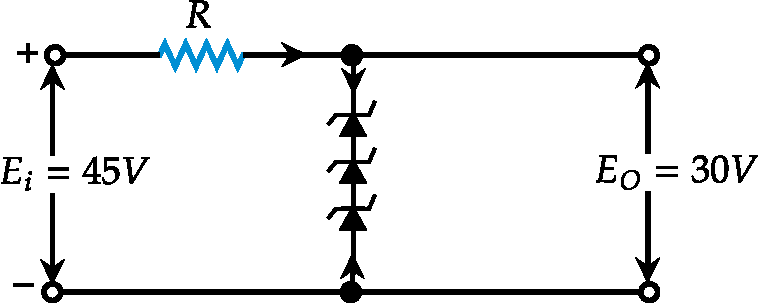
\includegraphics[height=3cm,width=6cm]{zener 2}
	
\end{figure}
\end{exercise}
\begin{answer}
	\begin{align*}
\text{	Regulated output voltage} \ E_0&=10+10+10=30\\
	\text{Voltage across}\ R&=E_i-E_0=45-30=15V\\
	R&=\frac{15v}{1000mA}=15\Omega
	\text{Since there is no load resistance } I&=I_Z
	\end{align*}

\end{answer}
\section{Diode applications}
\subsection{Series and parallel combination of diodes (problems)}
\begin{exercise}
Determine $I_D$,$V_{D_2}$ and $V_0$ for the circuit
\begin{figure}[H]
	\centering
	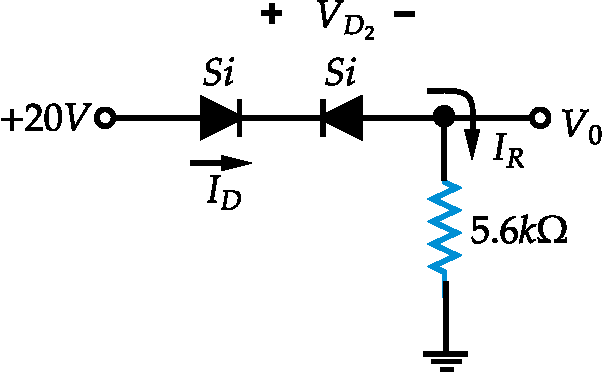
\includegraphics[height=3.5cm,width=5.5cm]{series}
\end{figure}
\end{exercise}
\begin{answer}
Since the second diode is reverse biased it will act as an open circiut.Then there will be no current flow through the circuit.therefore $I_D=0$(If $I_{D}$is zero $V_{D}$ will also be zero ).Then
$$I_{D_1}=0 \quad V_{D_1}=0$$
$$V_0=I_{R}	R=I_{D}R=0R=0V$$
Appliying kirchoff's law in a clockwise direction gives\\
$$E-V_{D_1}-V_{D_2}-V_0=0$$
$$V_{D_2}=E-V_{D_1}-V_0=20V-0-0=20V$$
\end{answer}
\begin{exercise}
Determine $V_0$,$I_1$,I$_{D_1}$ and $I_{D_2}$ for the parallel diode configuration:
\begin{figure}[H]
	\centering
	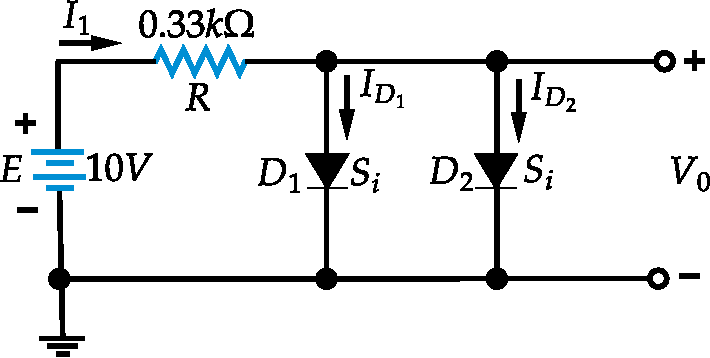
\includegraphics[height=3.5cm,width=6.5cm]{parallel 2}
\end{figure}	
\end{exercise}
\begin{answer}
Since the applied the two diodes are forward biased and the applied voltage is greater than 0.7V ,both diodes are in the ON state.The voltage across the parallel elements is always same
\begin{align*}
V_0&=0\\
\text{The current is,}
I_1&=\frac{E-V_D}{R}=\frac{10V-0.7V}{0.33k\Omega}=28.18mA
\intertext{Assuming diodes of similar characterestics, we have }
I_{D_1}&=I_{D_2}=\frac{I_1}{2}\\&=\frac{28.18}{2}=14.09mA
\end{align*}
\end{answer}
\subsection{OR and AND gates using diodes}
\begin{minipage}{0.5\textwidth}
\begin{figure}[H]
	\centering
	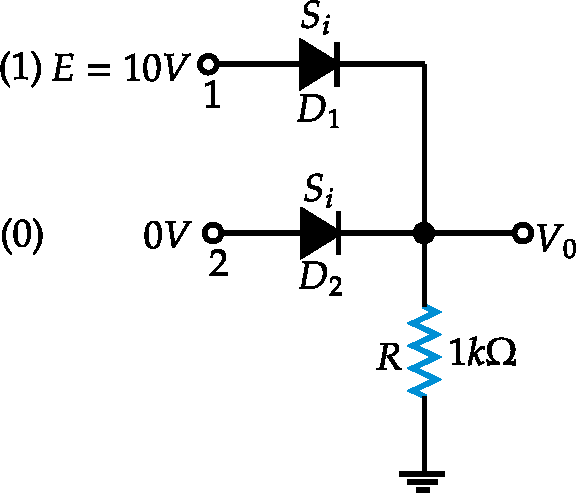
\includegraphics[height=4cm,width=4.5cm]{or}
	\caption{OR gate}
	\label{Diode OR gate}
	\end{figure}
\end{minipage}
\begin{minipage}{0.5\textwidth}
\begin{figure}[H]
	\centering
	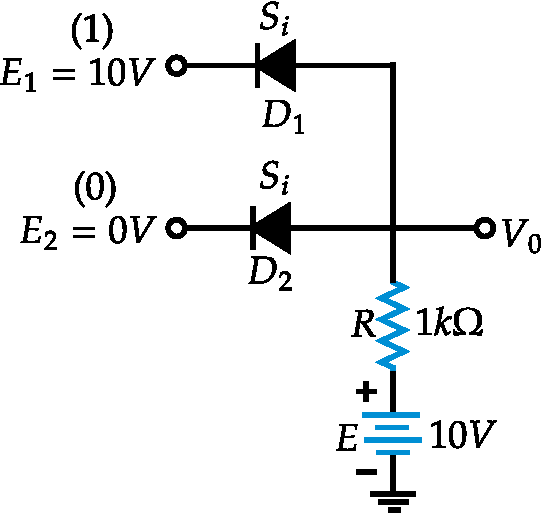
\includegraphics[height=4cm,width=4.5cm]{and}
	\caption{AND gate}
	\label{Diode AND gate}
\end{figure}
\end{minipage}\\\\
The figures.\ref{Diode AND gate} and \ref{Diode OR gate} shown are, OR and AND gate for positive logic.That is the 10V level of the figure is assigned as "1" for boolean algebra and 0V input is assigned as "0". An OR gate is such that the output voltage level will be a 1 if either or both input is a 1. The output ia a zero if both inputs are at the 0 level. An AND gate is such that the output voltage will be 1 only if the both inputs are high otherwise it will be zero.\\
The analysis of OR/AND gate is made easier by using an approximate equivalent for a diode rather than the ideal because we can stipulate that the voltage across the diode must be 0.7V positive for the siicon diode to switch to the ON state.
\section{Diode as rectifier}
The device which converts ac power into dc power by vertue of characterstic permitting appreciable flow of current in one direction only is called rectifier. Diode mcan be used as a rectifying elements in two different way.
\begin{enumerate}
	\item Half wave rectifier
	\item Full wave rectifier
\end{enumerate}
\subsection{Half wave rectification}
Over one full cycle,the average value (the algebraic sum of the areas above and below the axis) is zero. The circuit of Figure is called a half-wave rectifier, will generate a waveform $v_{o}$ that will have an average value for particular use. When employed in the rectification process, a diode is typically referred to as a rectifier. Its power and current ratings are typically much higher than those of diodes employed in other applications, such as computers and communication systems.
\begin{figure}[H]
\centering
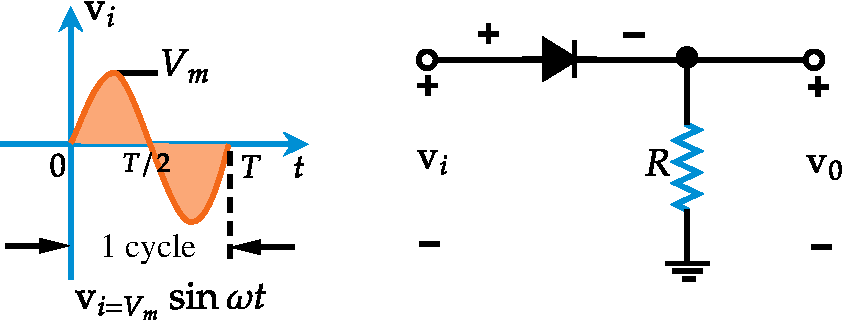
\includegraphics[height=3.8cm,width=9.3cm]{half}
\caption{}
\label{}
\end{figure}
 During the interval $t=0 \rightarrow T / 2$ in Figure the polarity of the applied voltage $v_{i}$ is such as to establish a forward current across the resisitor.The output signal is an exact replica of the applied signal. \\
For the period $T / 2 \rightarrow T$, the polarity of the input $v_{i}$ is such that the ideal diode produces an "off" state with an open-circuit equivalent. The result is the absence of a path for charge to flow, and $v_{o}=i R=(0) R=0 \mathrm{~V}$ for the period $T / 2 \rightarrow T$. \\
The input $v_{i}$ and the output $v_{o}$ are sketched together in Figure for comparison purposes.
\begin{figure}[H]
\centering
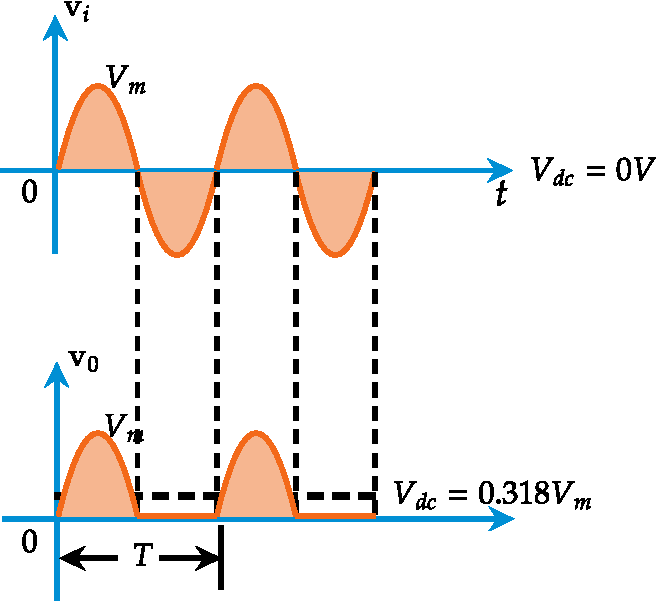
\includegraphics[height=6cm,width=8cm]{half graph}
\caption{}
\label{}
\end{figure}
The output signal $v_{o}$ now has a net positive area above the axis over a full period and an average value determined by 
$$V_{\mathrm{dc}}=0.318 V_{m}\quad \text{for half-wave rectifier }$$
When we consider the effect of using silicon diode with $V_k=0.7V$
$$V_{\mathrm{dc}} \cong 0.318\left(V_{m}-V_{K}\right)$$
\begin{note}
\begin{itemize}
	\item An ac voltage is applied with a wave frequency $\omega$ and peak current $I_{0}$ .
	\item Hence the current through the diode and load R, will be given by
	$$\begin{aligned}
	i &=I_{0} \sin \omega t \text { for } 0 \leq \omega t \leq \pi \\
	&=0 \text { for } \pi \leq \omega t \leq 2 \pi
	\end{aligned}$$
	\item
	$$ \begin{aligned}
	&I_{\text {d.c. }}=\frac{1}{2 \pi} \int_{0}^{2 \pi} i d(\omega t)=\frac{I_{0}}{\pi} \quad V_{\text {d.c. }}=\frac{I_{0} R_{L}}{\pi} \\
	&I_{\text {r.m.s. }}=\sqrt{\frac{1}{2 \pi} \int_{0}^{2 \pi} i^{2} d(\omega t)}=\frac{I_{0}}{2}
	\end{aligned}
	$$
	\item An important quantity called efficiency of rectification $(\eta) $is defined as
	$$
	\eta=\frac{P_{\mathrm{d} . \mathrm{c}}}{P_{\text {in }}} \times 100 \%=\frac{I_{\text {d.c. }}^{2} R_{L}}{I_{\text {r.m.s. }}^{2}\left(R_{f}+R_{L}\right)}=\frac{40.6}{\left(1+\frac{R_{f}}{R_{L}}\right)} \%
	$$
	where, $R_{f}$ is diode forward biased resistance.
	\item Another important quantity is ripple factor. 
	$$\begin{aligned}
	r&=\frac{\text { r.m.s. value of a.c. components of load current (or voltage) }}{\text { d.c. value of load current (or voltages) }}\\
	&=\frac{I_{\text {r.m. } .}}{I_{\text {d.c. }}}\\&=\frac{\sqrt{I_{\text {r.m.s. }}^{2}-I_{\text {d.c. }}^{2}}}{I_{\text {d.c. }}}\\&=\sqrt{\left(\frac{I_{\text {r.ms. }}}{I_{\text {d.c. }}}\right)^{2}-1}=1.21
	\end{aligned}
	$$
\end{itemize}
\end{note}
\subsection{PIV(PRV)}
The peak inverse voltage rating of the diode is of primary importance in the design of rectificaton process.Recall that it is the voltage rating that must not be exceeded in the reverse bias region or the diode will enter the zener avalanche region.It is fairly obvious that the PIV rating of the diode must equal or exceed the peak value of the applied voltage.Therefore,
\begin{center}
PIV rating$\geqq V_m$
\end{center}         
\subsection{Full wave rectification} 

\textbf{1.Center-Taped tranasformer}
\begin{figure}[H]
\centering
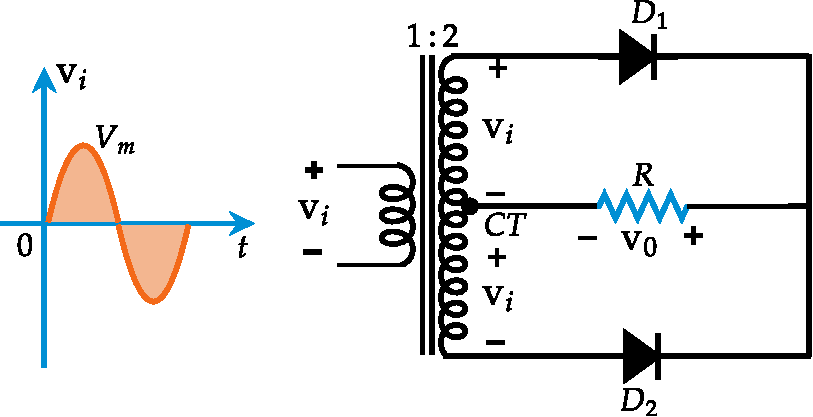
\includegraphics[height=5cm,width=9cm]{CT}
\caption{}
\label{}
\end{figure}
A second popular full-wave rectifier appears in Figure with only two diodes but requiring a center-tapped (CT) transformer to establish the input signal across each section of the secondary of the transformer. During the positive portion of $v_{i}$ applied to the primary of the transformer, the network will appear as shown  with a positive pulse across each section of the secondary coil. $D_{1}$ assumes the short-circuit equivalent and $D_{2}$ the open-circuit equivalent, as determined by the secondary voltages and the resulting current directions. The output voltage appears as in the case of bridge rectifier.
\par During the negative potion of te input it reverses the role of the diode but maintaining the same polarity for the voltage across the resisitor R.The net effect is shown bellow.
\begin{figure}[H]
\centering
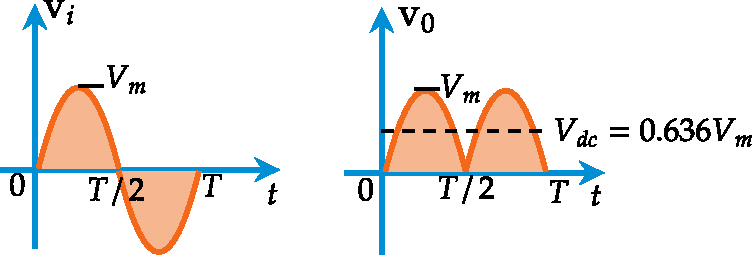
\includegraphics[height=3.2cm,width=9cm]{full graph}
\caption{}
\label{}
\end{figure}
Since the area above the axis for one full cycle is now twice that obtained for a full wave system,the dc level has also been doubled and 
$$V_{dc}=2 (0.318V_m)$$
$$V_{dc}=0.636V_m$$
If silicon rather than ideal diodes are employed 
$$V_{dc}=0.636(V_m-2V_k)$$
\begin{note}
\begin{itemize}
	\item For $0\leq \omega \leq \pi$
	$$\begin{aligned}
	&i_{1}=I_{0} \sin \omega t \\
	&i_{2}=0
	\end{aligned}
	$$
	For $\pi \leq\omega t\leq 2\pi$
	$$\begin{aligned}
	&i_{1}=0 \\
	&i_{2}=-I_{0} \sin \omega t
	\end{aligned}$$
	Where $i_{1}$ and $i_{2}$ are the current through the diodes $D_{1}$ and $D_{2}$
	\item $\begin{aligned}
	&I_{\text {d.c. }}=\frac{2 I_{0}}{\pi}, V_{\text {d.c. }}=\frac{2 I_{0} R_{L}}{\pi} \\
	&I_{\text {r.m.s. }}=\frac{I_{0}}{\sqrt{2}}
	\end{aligned}$
	\item Efficiency of rectification 
	$$\eta=\frac{I_{\mathrm{d} . \mathrm{c}}^{2} R_{L}}{I_{\mathrm{r} . \mathrm{m} . \mathrm{s}}^{2}\left(R_{f}+R_{L}\right)} \times 100 \%=\frac{81.2}{\left(1+\frac{R_{f}}{R_{L}}\right)} \%$$
	\item Ripple factor
	$$r=\sqrt{\frac{\left(I_{\text {r.m. } .}\right)^{2}}{I_{\text {d.c. }}^{2}}-1}=0.48$$
\end{itemize}
\end{note}
\subsubsection{PIV}
Inserting the maximum voltage for the secondary voltage and $V_{m}$ as established by the adjoining loop results in\\
\begin{minipage}{0.5\textwidth}
$$
\begin{aligned}
\mathrm{PIV} &=V_{\text {secondary }}+V_{R} \\
&=V_{m}+V_{m}\\
\text{and } \ \mathrm{PIV} &\geqq 2 V_{m} \quad \mathrm{CT} \text{ transformer, full-wave rectifier }
\end{aligned}
$$
\end{minipage}
\begin{minipage}{0.5\textwidth}
\begin{figure}[H]
	\centering
	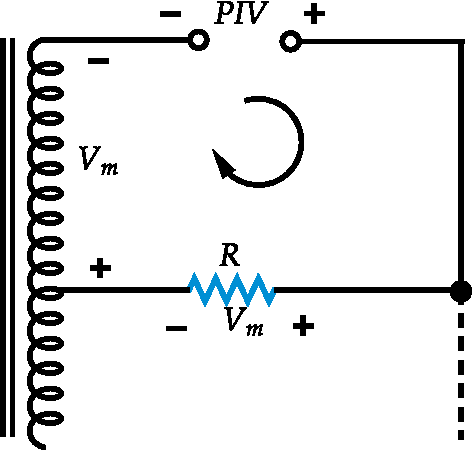
\includegraphics[height=4cm,width=4cm]{PIV2}
	\caption{}
	\label{}
\end{figure}
\end{minipage}
\textbf{2.Bridge network}
The dc level obtained from a sinusoidal input can be improved 100$\%$ using a process called full wave rectification.The most familiar network for performing such a function with four diode is bridge configuration.A full wave bridge rectifier is shown in the figure.
\begin{figure}[H]
\centering
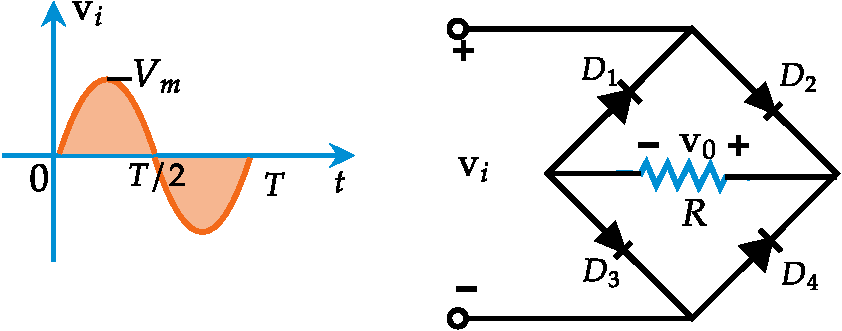
\includegraphics[height=3.5cm,width=9cm]{full}
\caption{}
\label{}
\end{figure}
During the period $t=0$ to $T/2$ polarity of the input wave the diodes $D_2$ and $D_3$ are conducting whereas $D_1$ and $D_4$ are in the off state.
\\ For the negative region of the input the diodes $D_1$ and $D_4$ are conducting and $D_2$ and $D_3$ are in OFF state.
Thus output has both positive and negative region.
\begin{note}
\begin{itemize}
	\item In bridge rectifier circuit a transformer with out center tap at the secondary is used.\\
	\item The expression for $I_{dc},I_{rms},\eta$ and r all are same except $R_{f}$ is now changed by 2$R_{f}$ ,since two diodes are conducting at a time.
\end{itemize}
\end{note}
\paragraph{PIV}
The required PIV of the each diode can be determined from figure obtained at the peak of the positive region of the input signal.For the indicated loop the maximum voltage across R is $V_m$ and the PIV rating is defined by
\begin{minipage}{0.5\textwidth}
\begin{center}
	PIV$\geqq V_m$ 
\end{center}
\end{minipage}
\begin{minipage}{0.5\textwidth}
\begin{figure}[H]
	\centering
	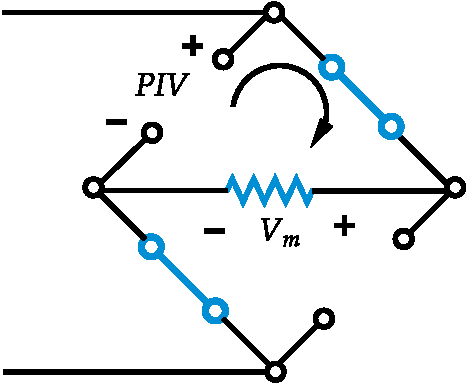
\includegraphics[height=4cm,width=5cm]{PIV1}
	\caption{}
	\label{}
\end{figure}
\end{minipage}
\begin{exercise}
A bridge rectifier feeds a load resistance of $2500 \Omega$ from a $30 \mathrm{~V}$ (rms) supply. Each diode of the rectifier has a forward resistance of $50 \Omega$. Calculate\\
(i) the dc load voltage\\
(ii) the ripple voltage at the output.
\end{exercise}
\begin{answer}
(i) The bridge circuit gives full wave rectification. So, the dc load current is $I_{\text {d.c. }}=\frac{2 I_{0}}{\pi}$, where $I_{0}$ is the peak load current. Since two diodes in serier conduct simultaneously, we have
$$
\begin{aligned}
&I_{0}=\frac{V_{0}}{2 R_{f}+R_{L}}=\frac{30 \sqrt{2}}{2 \times 50+2500}=0.0163 \mathrm{~A} \\
&\therefore I_{\text {d.c. }}=\frac{2 I_{\text {r.m.s. }}}{\pi}=0.0104 \mathrm{~A}
\end{aligned}
$$
The dc load voltage is $V_{\text {d.c. }}=I_{\text {d.c. }} R_{L}=0.0104 \times 2500=26 \mathrm{~V}$\\
(ii) The ripple voltage at the output is $I_{\mathrm{r} . \mathrm{m} . \mathrm{s}}^{\prime} R_{L}=\left(I_{\mathrm{r}, \mathrm{m} . \mathrm{s} .}^{2}-I_{\mathrm{d} . \mathrm{c} .}^{2}\right)^{1 / 2} R_{L}$
$$
\begin{aligned}
&I_{\text {rm. } .}=\frac{I_{0}}{\sqrt{2}}=0.0115 \mathrm{~A} \\
&\therefore I_{\mathrm{r}, \mathrm{m} . \mathrm{s}}^{\prime} R_{L}=\left(0.0115^{2}-0.0104^{2}\right)^{1 / 2} \times 2500=12.3 \mathrm{~V}
\end{aligned}
$$
\end{answer}
\section{Diode as clippers} 
Clippers are networks that employ diodes to "clip" away a portion of an input signal without distorting the remaining part of the applied waveform.\\
Halfwave rectifier is the simplest form of diode clipper-one resistor and a diode.Depending on the orientation of the diode,the positive and negative region of the applied voltage is clipped off.\\
There are two general cataegories of clippers :series and parallel.The series configuration is defind as one where the diode is in series with load,whereas the parallel variety has the diode in a branch parallel to the load.
\subsection{Series clippers}
Series clippers are again classified in to two.
\begin{enumerate}
	\item Series biased clippers
	\item Series unbiased clippers
\end{enumerate}
\subsubsection{Series unbiased clippers}
\begin{figure}[H]
\centering
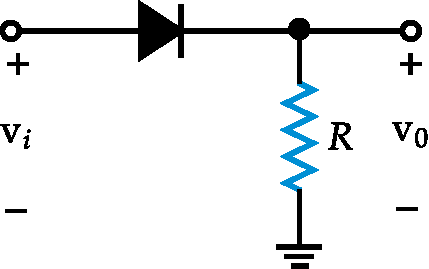
\includegraphics[height=3cm,width=4.5cm]{clip}
\caption{Series unbiased clipper}
\label{Series unbiased clipper}
\end{figure} 
The figure .\ref{Series unbiased clipper} shows the circuit of a negative clipper.Here the only voltage is the applied signal voltage and the output follows the input.There is a slight shift in the output voltage if we consider a practical diode instead of ideal one(Because the input voltage have to overcome the barrier potential(0.7V for silicon) in the case of a practical diode.)
\begin{figure}[H]
\centering
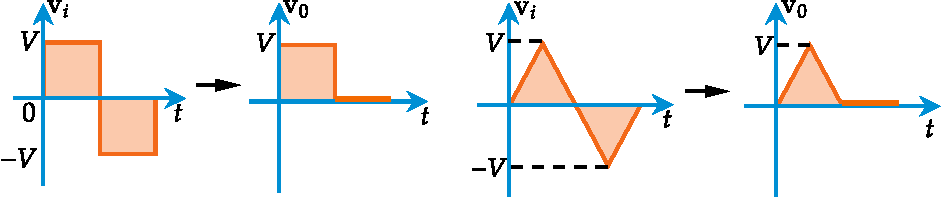
\includegraphics[height=3cm,width=12cm]{CLIPPER}
\caption{The negative clipper output of a square and triangular wave}
\label{}
\end{figure}
\subsubsection{Series biased clippers} 
The addition of dc supply to the network can have a prounced effect on the analysis of a series clipper ciruit.The dc supply can aid or work against the source voltage.\\\\
\textbf{CASE (I)} \textbf{When supply voltage is against the source voltage}
\begin{figure}[H]
\centering
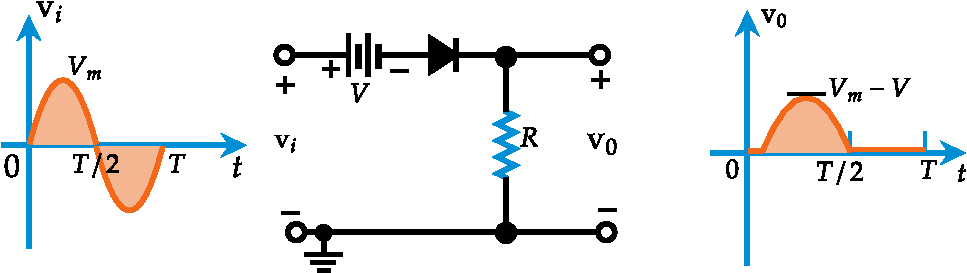
\includegraphics[height=3cm,width=10cm]{clip2}
\caption{}
\label{}
\end{figure}
Here $v_{i}$ is the source voltage and V is the supply voltage.When $v_{i}<V$ The diode will not conduct because it is reverse biased.And the output voltage $V_{0}$ is zero.And the clipper is said to be in OFF state.\\
When the applied voltage is greater than the supply voltage V.The diode is forward biased and the output voltage will be 
$$V_{0}=v_{i}-V$$
The diode is said to be ON state.\\
If $V_{m}$ is the peak voltage of input signal then\\
$$V_{0}=V_{m}-V$$
Here the the circuit is a negative clipper(ie it clipped off the negative portion)\\
A positive cipper can be formed be by reversing the direction of the diode and the source battery.\\
Here the output voltage will be \\
$$V_{0}=-(V_{m}-V)$$
\textbf{CASE (II)} \textbf{When supply voltage is aids the source voltage}
\begin{figure}[H]
\centering
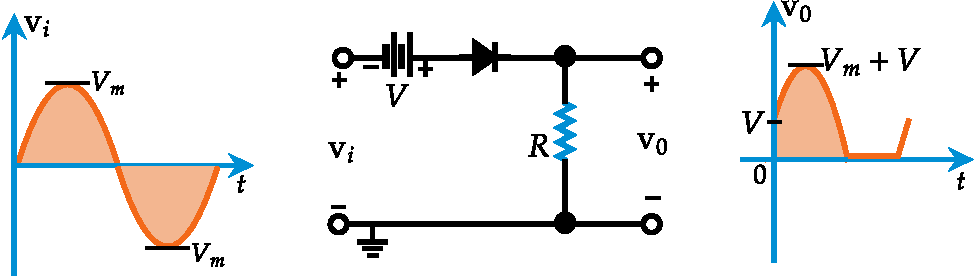
\includegraphics[height=3cm,width=10cm]{clip3}
\caption{}
\label{}
\end{figure}
Here the supply voltage makes the diode forward biased. During the positive half cycle of the input voltage the voltage across the diode will be equal to the some of the input voltage and the source voltage.The output voltage will be 
$$V_{0}=V_{m}+V$$
During the negative half cycle of the input voltage the diode will be in reverse biased if $V_{m}>V$.Since the the supply makes the diode forward biased always,during the negative half cycle a current will flow until the negative voltage overcome the supply voltage.\\
Here the circuit is a negative clipper.We wii get positive clipper  if we reverse the polarity of diode and source battery.And the output voltage will be 
$$V_{0}=-(V_{m}+V)$$
\subsection{Parallel clippers}
Which are again classified in to two
\begin{enumerate}
	\item Parellel unbiased clippers
	\item Parellel biased clippers
\end{enumerate}

\subsubsection{Parallel unbiased clippers}
\begin{figure}[H]
\centering
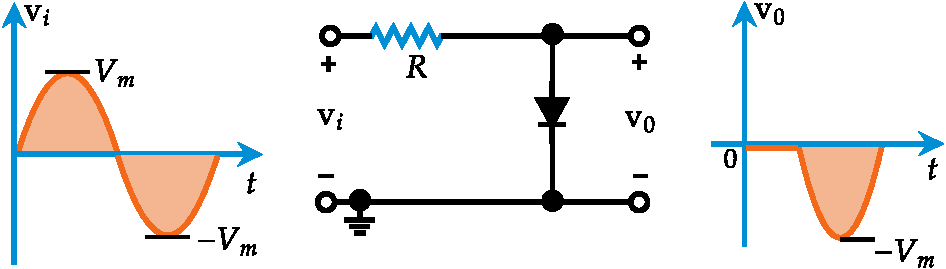
\includegraphics[height=3cm,width=8.5cm]{parallel b}
\caption{}
\label{}
\end{figure}
The network is the simplest of parallel diode configuration with the output for the same input.The analysis of parallel configuration is very similar to that applied  series configuration.During the positive half cycle of input the diode become in ON state.Then the current will flow through the loop.No current will appear at the output.During the negative half cycle the diode will act as an open circuit and the input voltage will appear across the output and output varries in accordance with the input.
\subsubsection{Parallel biased clippers}
\begin{figure}[H]
\centering
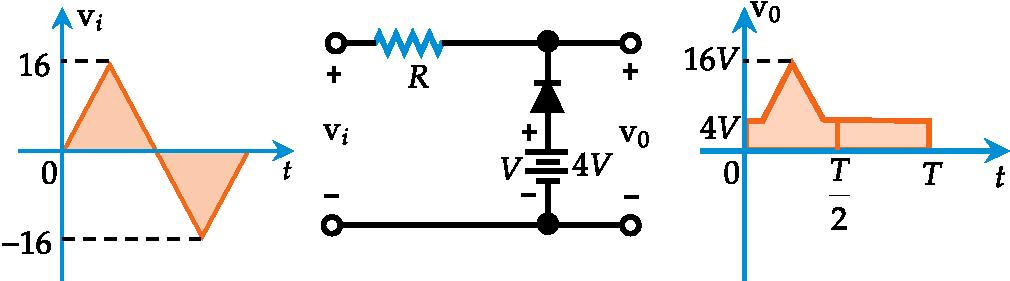
\includegraphics[height=3cm,width=11cm]{parallel ub}
\caption{}
\label{}
\end{figure}
From the figure we can say that there is always a +4V appears across the output because the output is parallel with the supply.During the positive half cycle the diode become reverse biased and no current will flow through the loop.The voltage across the input completely appears at the output.The output varries in accordamce with the input.But during the negative portion of the input signal the diode become ON state and a current will flow through the loop and no current will flow through the output after the negative voltage starts.
\begin{example}
\end{example}
\begin{figure}[H]
\centering
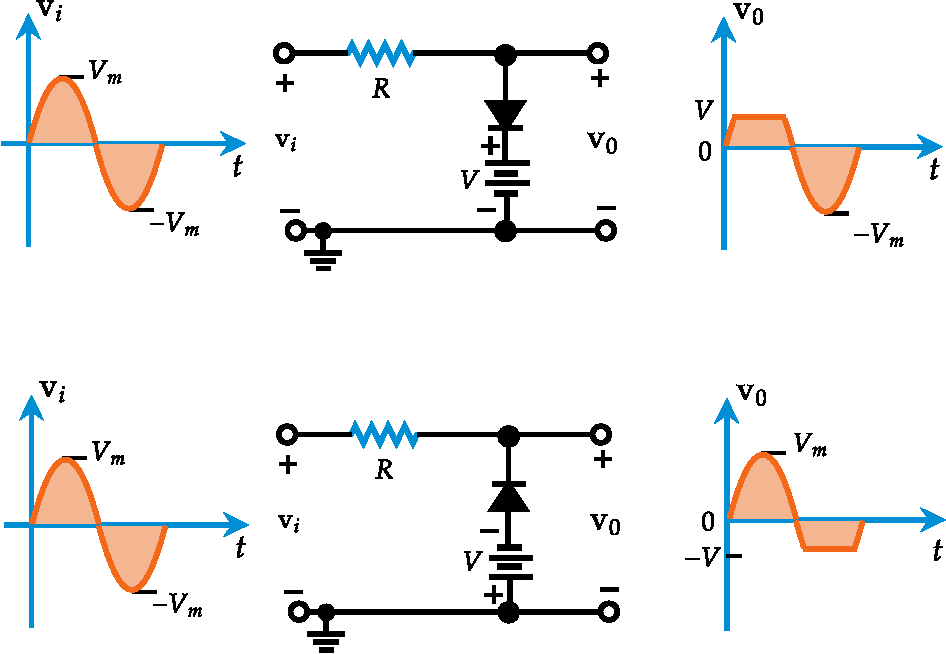
\includegraphics[height=7cm,width=10cm]{diagram-20211105(8)-crop}
\caption{}
\label{}
\end{figure}
\begin{example}
\end{example}
\begin{figure}[H]
\centering
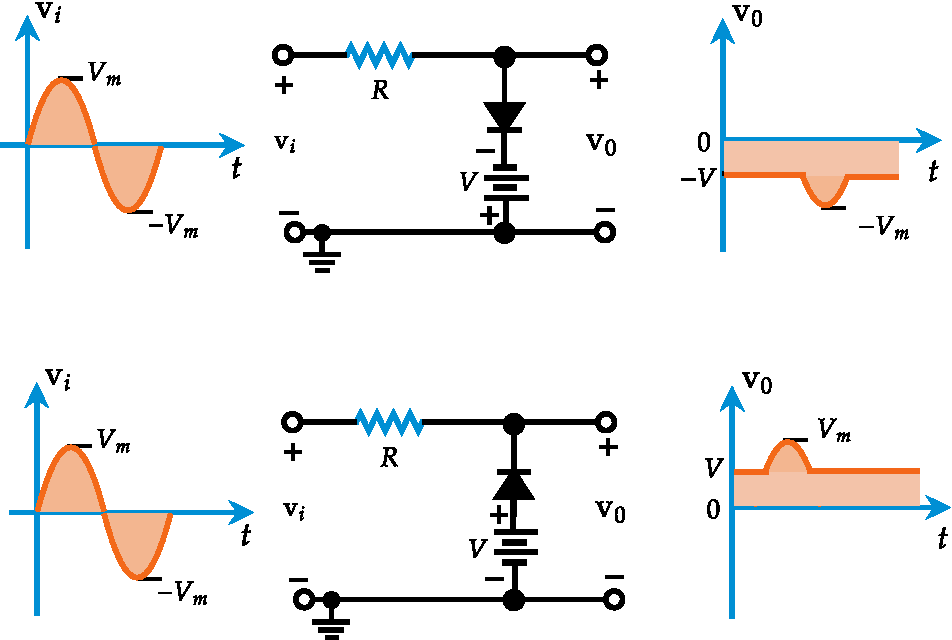
\includegraphics[height=7cm,width=10cm]{diagram-20211105(9)-crop}
\caption{}
\label{}
\end{figure}
\subsection{Clampers}
A clamper is a network constructed of a diode,a resistor and a capacitor that shifts a waveform to a different dc level without changing the appearance of the applied signal. Clamping network have a capacitor connected directly from input to output with a resistive element in parallel with the output signal.The diode is also parallel with the output signal but may or may not have a series dc supply as an added element. There is a sequence of steps that can be applied to help make the analysis stright forward\\
\textbf{Step 1: } Start the analysis by examining the responsse of the portion of the input signal that will forward bias the diode.\\
\textbf{Step 2: } During the period that the diode is in "on" state,assume the capacitor will charge up instantaneously to a voltage level determined by the surrounding network.\\
\textbf{Step 3: } Assume that during the period when the diode is in the "off" state the capacitor hold on to its established voltage level.\\
\textbf{Step 4: } Throughout the analysis maintain a contenual awareness of the location and defind polarity for $v_{0}$ to ensure that the proper levels are obtained.\\
\textbf{Step 5: } Check that the total swing of the output matches that of the input.
\begin{exercise}
Determine the $v_{0}$ for the network for the input indicated:
\end{exercise}
\begin{answer}$\left. \right. $
\begin{figure}[H]
	\centering
	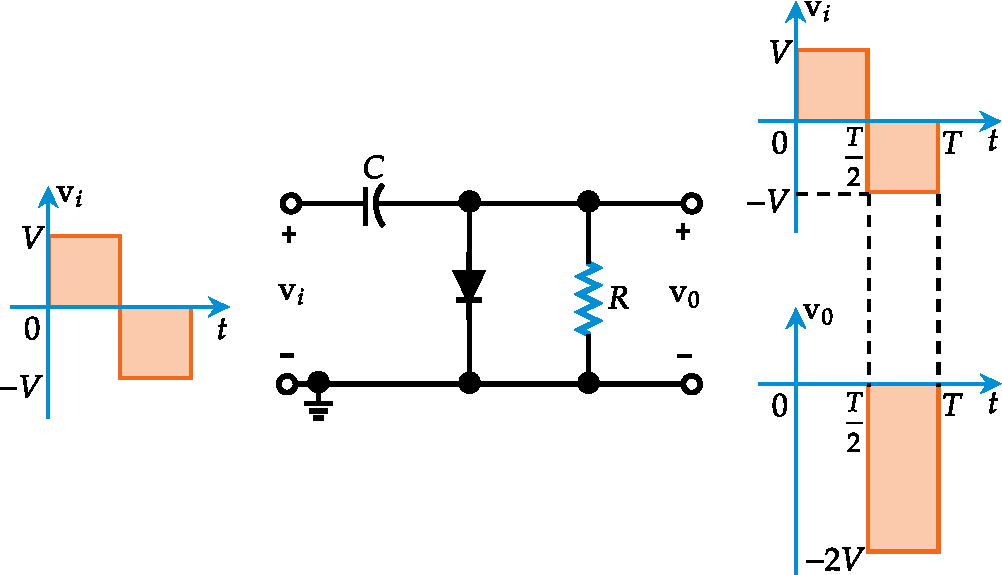
\includegraphics[height=6cm,width=10cm]{diagram-20211103-crop(1)}
\end{figure}
The diode will be forward biased for the positive portion of the applied signal.The short circuit equivalent for the diode will result in $v_{0}=0$ for this time interval.During this time the time constant will be small$(\tau=RC)$ because no current will flow through the resistor(resistance equal to the resisitance of the wire only).The result is that the capacitor will quickly charge to the peak value of V volts.Thus the voltage drop across the capacitor is equal to V volts.
\\ When the input swiches to the $-V$ state .The diode become open circuited and the output voltage across the resistor is found out by applying kirchoff's voltage law to the loop in clockwise direction.Which will be equal to sum of voltage across the resisitor(-V) and the input voltage(-V) ie -2V.
$$V_{0}=-2V$$
During the negative half cycle the resistor is included in the circuit.so time constant ($\tau=RC$) will be a large value.It will be greater than the time period $\frac{T}{2}$ so it will not dicharged out before the next cycle arrives.The output can be drwan as shown in thefigure.
\end{answer}
\section{Clampers examples}
\begin{example}$\left. \right. $\\
	\begin{figure}[H]
		\centering
		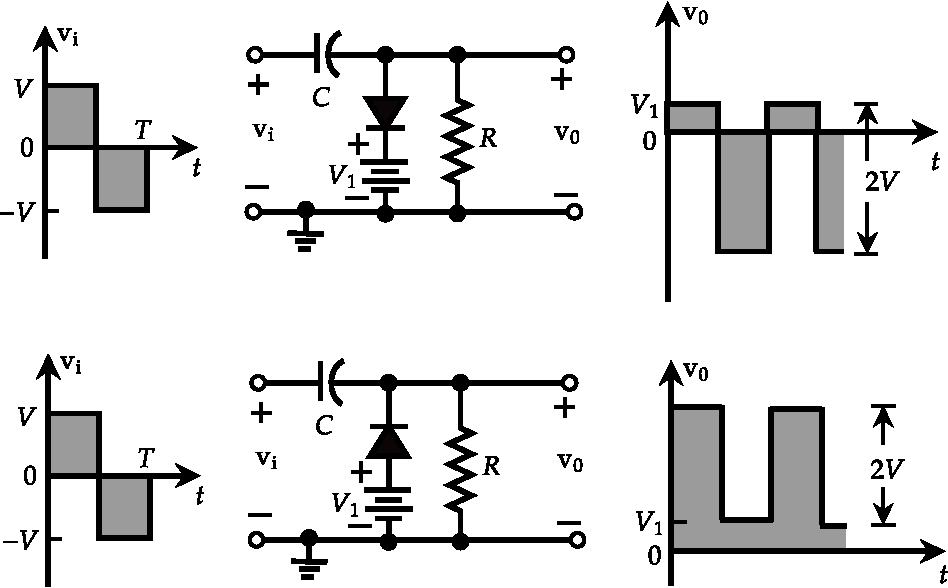
\includegraphics[height=6cm,width=9cm]{diagram-20211104(7)-crop}
	\end{figure}
\end{example}
 
\begin{example}$\left. \right. $\\
\begin{figure}[H]
\centering
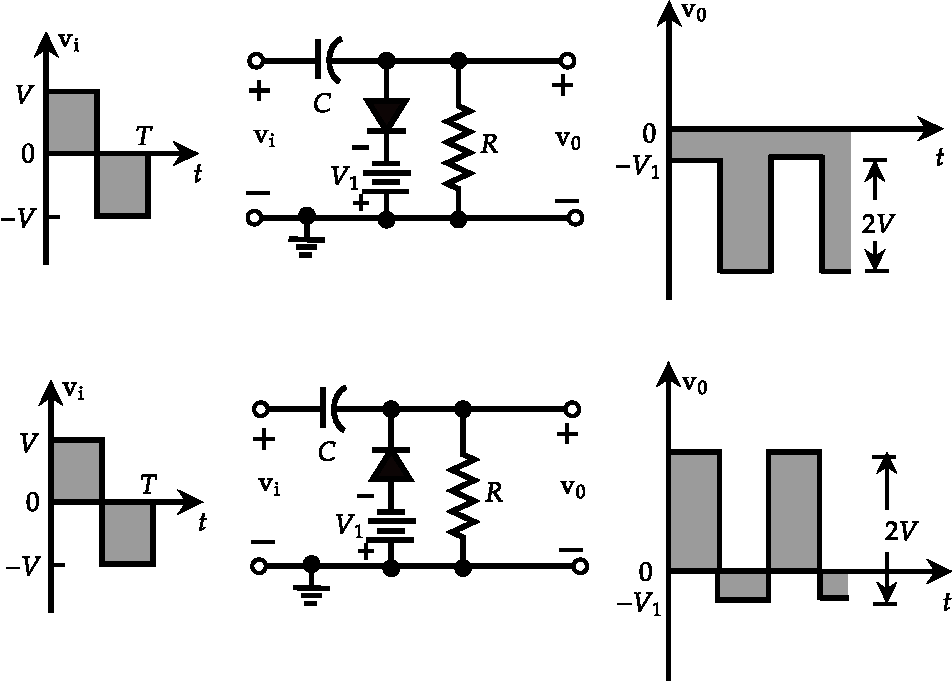
\includegraphics[height=6cm,width=9cm]{diagram-20211104(9)-crop}
\end{figure}
\end{example}
\begin{example}$\left. \right. $\\
\begin{figure}[H]
\centering
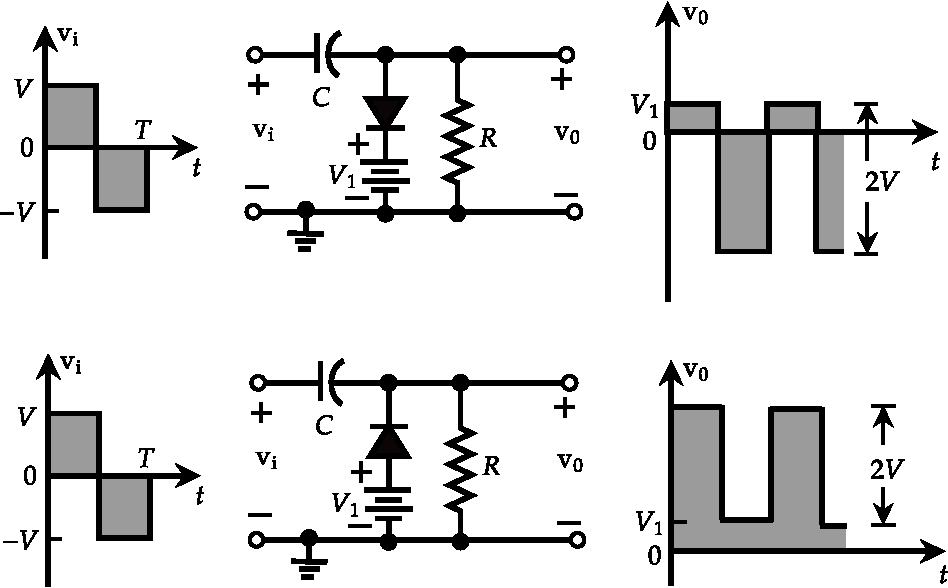
\includegraphics[height=6cm,width=9cm]{diagram-20211104(8)-crop}
\end{figure}
\end{example}

\newpage
\begin{abox}
	Practise Set-1
\end{abox}
\begin{enumerate}
	\item An LED operates at $1.5 \mathrm{~V}$ and $5 \mathrm{~mA}$ in forward bias. Assuming an $80 \%$ external efficiency of the LED, how many photons are emitted per second?
	{	\exyear{NET/JRF(JUNE-2012)}}
	\begin{tasks}(4)
		\task[\textbf{A.}] $5.0 \times 10^{16}$
		\task[\textbf{B.}]  $1.5 \times 10^{16}$
		\task[\textbf{C.}] $0.8 \times 10^{16}$
		\task[\textbf{D.}] $2.5 \times 10^{16}$
	\end{tasks}
	\item A sample of $S i$ has electron and hole mobilities of $0.13$ and $0.05 \mathrm{~m}^{2} / \mathrm{V}-\mathrm{s}$ respectively at $300 \mathrm{~K}$. It is doped with $P$ and $A l$ with doping densities of $1.5 \times 10^{21} / \mathrm{m}^{3}$ and $2.5 \times 10^{21} / \mathrm{m}^{3}$ respectively. The conductivity of the doped Si sample at $300 \mathrm{~K}$ is
	{	\exyear{NET/JRF(DEC-2013)}}
	\begin{tasks}(4)
		\task[\textbf{A.}] $8 \Omega^{-1} m^{-1}$
		\task[\textbf{B.}] $32 \Omega^{-1} m^{-1}$
		\task[\textbf{C.}] $20.8 \Omega^{-1} m^{-1}$
		\task[\textbf{D.}] $83.2 \Omega^{-1} m^{-1}$
	\end{tasks}
	\item Two identical Zener diodes are placed back to back in series and are connected to a variable DC power supply. The best representation of the $I-V$ characteristics of the circuit is
	{	\exyear{NET/JRF(DEC-2013)}}
	\begin{tasks}(2)
		\task[\textbf{A.}] \begin{figure}[H]
			\centering
			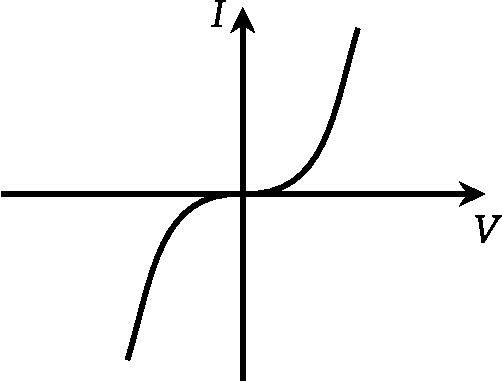
\includegraphics[height=3.5cm,width=4cm]{e-24a}
		\end{figure}
		\task[\textbf{B.}] \begin{figure}[H]
			\centering
			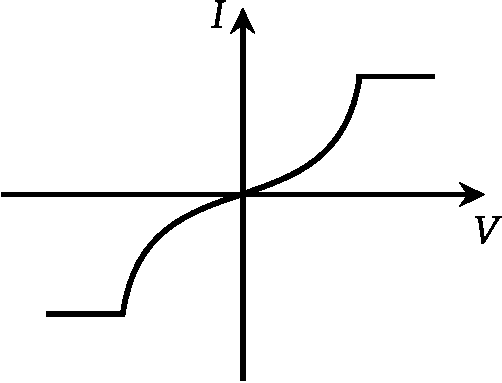
\includegraphics[height=3.5cm,width=4cm]{e-24b}
		\end{figure}
		\task[\textbf{C.}] \begin{figure}[H]
			\centering
			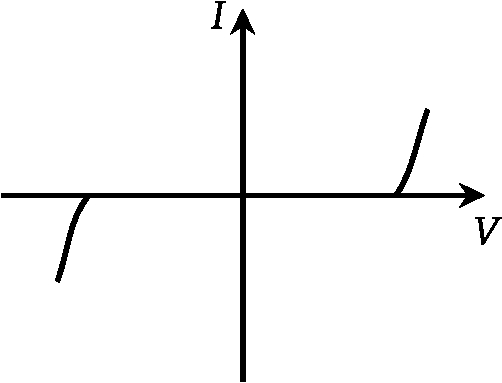
\includegraphics[height=3.5cm,width=4cm]{e-24c}
		\end{figure}
		\task[\textbf{D.}] \begin{figure}[H]
			\centering
			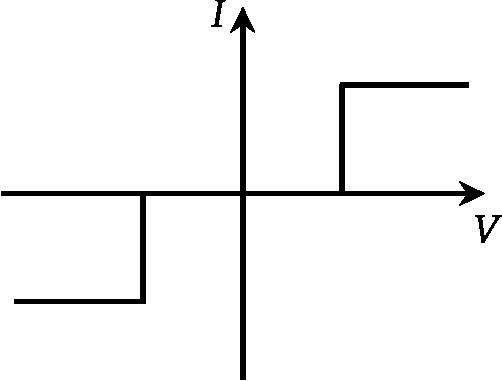
\includegraphics[height=3.5cm,width=4cm]{e-24d}
		\end{figure}
	\end{tasks}
	\item The power density of sunlight incident on a solar cell is $100 \mathrm{~mW} / \mathrm{cm}^{2}$. Its short circuit current density is $30 \mathrm{~mA} / \mathrm{cm}^{2}$ and the open circuit voltage is $0.7 \mathrm{~V}$. If the fill factor of the solar cell decreases from $0.8$ to $0.5$ then the percentage efficiency will decrease from
	{\exyear{NET/JRF(DEC-2014)}}
	\begin{tasks}(4)
		\task[\textbf{A.}] $42.0$ to $26.2$
		\task[\textbf{B.}] $24.0$ to $16.8$
		\task[\textbf{C.}] $21.0$ to $10.5$
		\task[\textbf{D.}] $16.8$ to $10.5$
	\end{tasks}
	\item The concentration of electrons, $n$ and holes $p$, for an intrinsic semiconductor at a temperature $T$ can be expressed as $n=p=A T^{\frac{3}{2}} \exp \left(-\frac{E_{g}}{2 k_{B} T}\right)$, where $E_{g}$ is the band gap and $A$ is a constant. If the mobility of both types of carrier is proportional to $T^{\frac{-3}{2}}$, then the log of the conductivity is a linear function of $T^{-1}$, with slope
	{	\exyear{NET/JRF(JUNE-2015)}}
	\begin{tasks}(4)
		\task[\textbf{A.}]$\frac{E_{g}}{\left(2 k_{B}\right)}$
		\task[\textbf{B.}] $\frac{E_{g}}{k_{B}}$
		\task[\textbf{C.}] $\frac{-E_{g}}{\left(2 k_{B}\right)}$
		\task[\textbf{D.}] $\frac{-E_{g}}{k_{B}}$
	\end{tasks}
	\item The decay constants $f_{p}$ of the heavy pseudo-scalar mesons, in the heavy quark limit, are related to their masses $m_{p}$ by the relation $f_{p}=\frac{a}{\sqrt{m_{p}}}$, where $a$ is an empirical parameter to be determined. The values $m_{p}=(6400 \pm 160) \mathrm{MeV}$ and $f_{p}=(180 \pm 15) \mathrm{MeV}$ correspond to uncorrelated measurements of a meson. The error on the estimate of $a$ is
	{	\exyear{NET/JRF(JUNE-2016)}}
	\begin{tasks}(4)
		\task[\textbf{A.}] $175(\mathrm{MeV})^{\frac{3}{2}}$
		\task[\textbf{B.}] $900(\mathrm{MeV})^{\frac{3}{2}}$
		\task[\textbf{C.}] $1200(\mathrm{MeV})^{\frac{3}{2}}$
		\task[\textbf{D.}] $2400(\mathrm{MeV})^{\frac{3}{2}}$
	\end{tasks}
	\item Let $I_{0}$ be the saturation current, $\eta$ the ideality factor and $v_{F}$ and $v_{R}$ the forward and reverse potentials respectively, for a diode. The ratio $R_{R} / R_{F}$ of its reverse and forward resistances $R_{R}$ and $R_{F}$, respectively, varies as (In the following $k_{B}$ is the Boltzmann constant, $T$ is the absolute temperature and $q$ is the charge.)
	{\exyear{NET/JRF(JUNE-2017)}}
	\begin{tasks}(2)
		\task[\textbf{A.}] $\frac{v_{R}}{v_{F}} \exp \left(\frac{q v_{F}}{\eta k_{B} T}\right)$
		\task[\textbf{B.}] $\frac{v_{F}}{v_{R}} \exp \left(\frac{q v_{F}}{\eta k_{B} T}\right)$
		\task[\textbf{C.}]  $\frac{v_{R}}{v_{F}} \exp \left(-\frac{q v_{F}}{\eta k_{B} T}\right)$
		\task[\textbf{D.}]  $\frac{v_{F}}{v_{R}} \exp \left(-\frac{q v_{F}}{\eta k_{B} T}\right)$
	\end{tasks}
	\item Both the data points and a linear fit to the current vs voltage of a resistor are shown in the graph below.\\
	\begin{figure}[H]
		\centering
		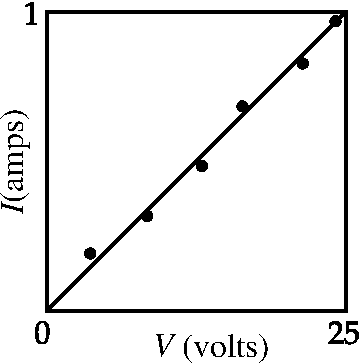
\includegraphics[height=4cm,width=4cm]{e59}
	\end{figure}
	If the error in the slope is $1.255 \times 10^{-3} \Omega^{-1}$, then the value of resistance estimated from the graph is
	{\exyear{NET/JRF(JUNE-2017)}}
	\begin{tasks}(4)
		\task[\textbf{A.}] $(0.04 \pm 0.8) \Omega$
		\task[\textbf{B.}] $(25.0 \pm 0.8) \Omega$
		\task[\textbf{C.}] $(25 \pm 1.25) \Omega$
		\task[\textbf{D.}] $(25 \pm 0.0125) \Omega$
	\end{tasks}
	\item A sinusoidal signal with a peak voltage $V_{p}$ and average value zero, is an input to the following circuit.\\
	\begin{figure}[H]
		\centering
		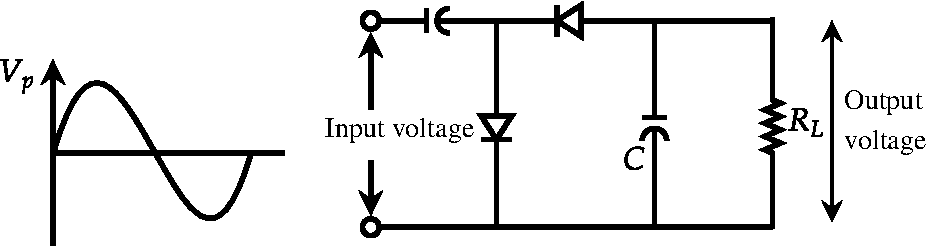
\includegraphics[height=2.5cm,width=9cm]{e67}
	\end{figure}
	Assuming ideal diodes, the peak value of the output voltage across the load resistor $R_{L}$ is
	{\exyear{NET/JRF(JUNE-2018)}}
	\begin{tasks}(4)
		\task[\textbf{A.}] $V_{p}$
		\task[\textbf{B.}] $\frac{V_{p}}{2}$
		\task[\textbf{C.}]  $2 V_{p}$
		\task[\textbf{D.}]  $\sqrt{2} V_{p}$
	\end{tasks}
	\item A sinusoidal voltage having a peak value of $V_ p$ is an input to the following circuit, in which the $DC$ voltage is $V_b$ \\
	\begin{figure}[H]
		\centering
		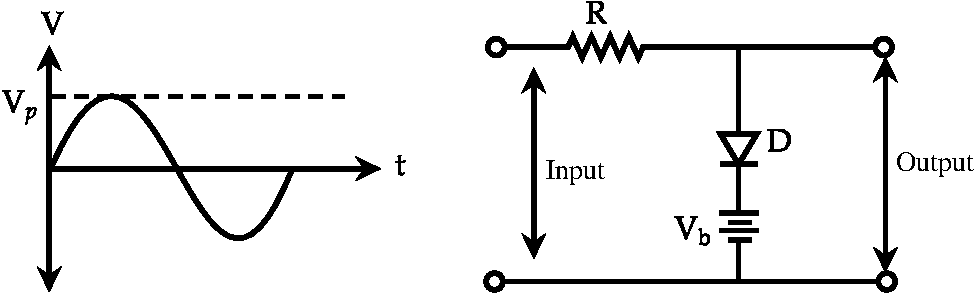
\includegraphics[height=3cm,width=9cm]{e77}
	\end{figure}
	Assuming an ideal diode which of the following best describes the output waveform?
	{\exyear{NET/JRF(DEC-2018)}}
	\begin{tasks}(2)
		\task[\textbf{A.}] \begin{figure}[H]
			\centering
			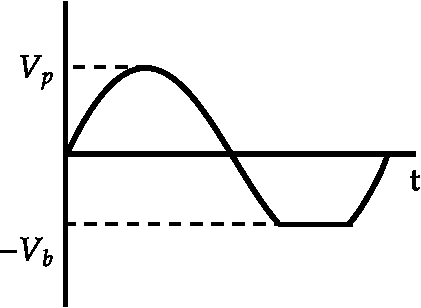
\includegraphics[height=3cm,width=4cm]{e77a}
		\end{figure}
		\task[\textbf{B.}] \begin{figure}[H]
			\centering
			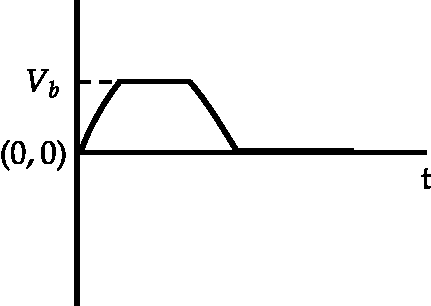
\includegraphics[height=3cm,width=4cm]{e77b}
		\end{figure}
		\task[\textbf{C.}] \begin{figure}[H]
			\centering
			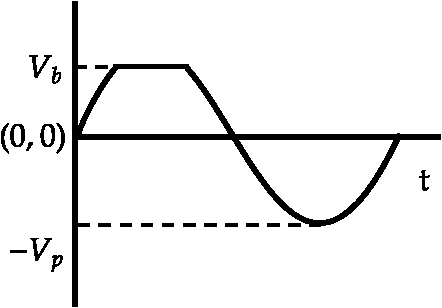
\includegraphics[height=3cm,width=4cm]{e77c}
		\end{figure}
		\task[\textbf{D.}] \begin{figure}[H]
			\centering
			\includegraphics[height=3cm,width=4cm]{e77d}
		\end{figure}
	\end{tasks}
	\item A $10 V$ battery is connected in series to a resistor $R$ and a capacitor $C$, as shown the figure.\\\begin{figure}[H]
		\centering
		\includegraphics[height=3cm,width=6cm]{BJT-1}
	\end{figure}
	The initial charge on the capacitor is zero. The switch is turned on and the capacitor is allowed to charge to its full capacity. The total work done by the battery in this process is
	{\exyear{NET/JRF(JUNE-2020)}}
	\begin{tasks}(4)
		\task[\textbf{A.}] $10^{-3} \mathrm{~J}$
		\task[\textbf{B.}] $2 \times 10^{-3} \mathrm{~J}$
		\task[\textbf{C.}] $5 \times 10^{-4} \mathrm{~J}$
		\task[\textbf{D.}] $47 \times 10^{-2} \mathrm{~J}$
	\end{tasks}
	\item The temperature variation of the resistivity of four materials are shown in the following graphs.
	\begin{tasks}(2)
		\task[\textbf{A.}] \begin{figure}[H]
			\centering
			\includegraphics[height=3cm,width=4cm]{BJT-02}
		\end{figure}
		\task[\textbf{B.}]\begin{figure}[H]
			\centering
			\includegraphics[height=3cm,width=4cm]{BJT-03}
		\end{figure}
		\task[\textbf{C.}] \begin{figure}[H]
			\centering
			\includegraphics[height=3cm,width=4cm]{BJT-04}
		\end{figure}
		\task[\textbf{D.}] \begin{figure}[H]
			\centering
			\includegraphics[height=3cm,width=4cm]{BJT-06}
		\end{figure}
	\end{tasks}
	The material that would make the most sensitive temperature sensor, when used at temperatures between $T_{1}$ and $T_{2}$, is
	{\exyear{NET/JRF(JUNE-2020)}}
	\begin{tasks}(4)
		\task[\textbf{A.}] A
		\task[\textbf{B.}] B
		\task[\textbf{C.}] C
		\task[\textbf{D.}] D
	\end{tasks}
	\item Two voltmeters $A$ and $B$ with internal resistances $2 M \Omega$ and $0.1 k \Omega$ are used to measure the voltage drops $V_{A}$ and $V_{B}$, respectively, across the resistor $R$ in the circuit shown below.\\
	\begin{figure}[H]
		\centering
		\includegraphics[height=2.5cm,width=6cm]{BJT-07}
	\end{figure}
	The ratio $V_{A} / V_{B}$ is
	{\exyear{NET/JRF(JUNE-2020)}}
	\begin{tasks}(4)
		\task[\textbf{A.}] $0.58$
		\task[\textbf{B.}] $1.73$
		\task[\textbf{C.}] 1
		\task[\textbf{D.}] 2
	\end{tasks}
	\item The $I-V$ characteristics of the diode $D$ in the circuit below is given by
	$$
	I=I_{s}\left(e^{\frac{q V}{k_{\mathrm{B}} T}}-1\right)
	$$
	where $I_{s}$ is the reverse saturation current, $V$ is the voltage across the diode and $T$ is the absolute temperature.\\
	\begin{figure}[H]
		\centering
		\includegraphics[height=3.5cm,width=6cm]{BJT-11}
	\end{figure}
	If the input voltage is $V_{\text {in }}$, then the output voltage $V_{\text {out }}$ is
	{\exyear{NET/JRF(JUNE-2020)}}
	\begin{tasks}(2)
		\task[\textbf{A.}] (a) $I_{s} R \ln \left(\frac{q V_{\text {in }}}{k_{B} T}+1\right)$
		\task[\textbf{B.}] $\frac{1}{q} k_{B} T \ln \left(\frac{q\left(V_{\text {in }}+I_{s} R\right)}{k_{B} T}\right)$
		\task[\textbf{C.}]  $\frac{1}{q} k_{B} T \ln \left(\frac{V_{\text {in }}}{I_{s} R}+1\right)$
		\task[\textbf{D.}]  $-\frac{1}{q} k_{B} T \ln \left(\frac{V_{\text {in }}}{I_{s} R}+1\right)$
	\end{tasks}
\end{enumerate}
\colorlet{ocre1}{ocre!70!}
\colorlet{ocrel}{ocre!30!}
\setlength\arrayrulewidth{1pt}
\begin{table}[H]
	\centering
	\arrayrulecolor{ocre}
	\begin{tabular}{|p{1.5cm}|p{1.5cm}||p{1.5cm}|p{1.5cm}|}
		\hline
		\multicolumn{4}{|c|}{\textbf{Answer key}}\\\hline\hline
		\rowcolor{ocrel}Q.No.&Answer&Q.No.&Answer\\\hline
		1&\textbf{D} &2&\textbf{A}\\\hline 
		3&\textbf{D} &4&\textbf{D} \\\hline
		5&\textbf{C} &6&\textbf{C} \\\hline
		7&\textbf{A}&8&\textbf{B}\\\hline
		9&\textbf{C}&10&\textbf{C}\\\hline
		11&\textbf{A} &12&\textbf{C}\\\hline
		13&\textbf{B}&14&\textbf{C}\\\hline
	\end{tabular}
\end{table}
\newpage
\begin{abox}
	Practise Set-2
\end{abox}
\begin{enumerate}
	\item For an intrinsic semiconductor, $m_{e}^{*}$ and $m_{h}^{*}$ are respectively the effective masses of electrons and holes near the corresponding band edges. At a finite temperature the position of the Fermi level
{	\exyear{GATE 2011}}
\begin{tasks}(2)
\task[\textbf{A.}] Depends on $m_{e}{ }^{*}$ but not on $m_{h}{ }^{*}$
\task[\textbf{B.}] Depends on $m_{h}{ }^{*}$ but not on $m_{e}{ }^{*}$
\task[\textbf{C.}] Depends on both $m_{e}{ }^{*}$ and $m_{h}{ }^{*}$
\task[\textbf{D.}] Depends neither on $m_{e}{ }^{*}$ nor on $m_{h}{ }^{*}$
\end{tasks}
	\item In the following circuit, the voltage across and the current through the $2 \mathrm{k} \Omega$ resistance are
{	\exyear{GATE 2011}}
\begin{figure}[H]
\centering
\includegraphics[height=4cm,width=9cm]{SC-1}
\end{figure}
\begin{tasks}(4)
\task[\textbf{A.}] $20 \mathrm{~V}, 10 \mathrm{~mA}$
\task[\textbf{B.}] $20 \mathrm{~V}, 5 \mathrm{~mA}$
\task[\textbf{C.}] $10 \mathrm{~V}, 10 \mathrm{~mA}$
\task[\textbf{D.}] $10 \mathrm{~V}, 5 \mathrm{~mA}$
\end{tasks}
	\item A Ge semiconductor is doped with acceptor impurity concentration of $10^{15}$ atoms $/ \mathrm{cm}^{3}$. For the given hole mobility of $1800 \mathrm{~cm}^{2} / \mathrm{V}$-s, the resistivity of the material is
{	\exyear{GATE 2012}}
\begin{tasks}(4)
\task[\textbf{A.}] $0.288 \Omega \mathrm{cm}$
\task[\textbf{B.}] $0.694 \Omega \mathrm{cm}$
\task[\textbf{C.}] $3.472 \Omega \mathrm{cm}$
\task[\textbf{D.}] $6.944 \Omega \mathrm{cm}$
\end{tasks}
	\item Identify the CORRECT energy band diagram for silcon doped with Arsenic. Here CB, VB, $E_{D}$ and $E_{F}$ are conduction band, valence band, impurity level and Fermi level, respectively.
{	\exyear{GATE 2012}}
\begin{tasks}(2)
\task[\textbf{A.}] \begin{figure}[H]
	\centering
	\includegraphics[height=4.5cm,width=5cm]{diagram-20210913(8)-crop}
\end{figure}
\task[\textbf{B.}] \begin{figure}[H]
	\centering
	\includegraphics[height=4.5cm,width=5cm]{diagram-20210913(9)-crop}
\end{figure}
\task[\textbf{C.}] \begin{figure}[H]
	\centering
	\includegraphics[height=4.5cm,width=5cm]{diagram-20210913(10)-crop}
\end{figure}
\task[\textbf{D.}] \begin{figure}[H]
	\centering
	\includegraphics[height=4.5cm,width=5cm]{diagram-20210913(11)-crop}
\end{figure}
\end{tasks}
	\item A phosphorous doped silicon semiconductor (doping density: $\left.10^{17} / \mathrm{cm}^{3}\right)$ is heated from $100^{\circ} \mathrm{C}$ to $200^{\circ} \mathrm{C}$. Which one of the following statements is CORRECT?
{	\exyear{GATE 2013}}
\begin{tasks}(1)
\task[\textbf{A.}] Position of Fermi level moves towards conduction band
\task[\textbf{B.}] Position of dopant level moves towards conduction band
\task[\textbf{C.}] Position of Fermi level moves towards middle of energy gap
\task[\textbf{D.}] Position of dopant level moves towards middle of energy gap
\end{tasks}
	\item The donor concentration in a sample of $n$-type silicon is increased by a factor of 100 . The shift in the position of the Fermi level at $300 \mathrm{~K}$, assuming the sample to non degenerate\\ is ----------$\mathrm{meV} . \quad\left(k_{B} T=25 \mathrm{meV}\right.$ at $\left.300 \mathrm{~K}\right)$
{	\exyear{GATE 2014}}
	\item The band gap of an intrinsic semiconductor is $E_{g}=0.72 \mathrm{eV}$ and $m_{h}^{*}=6 m_{n}^{*} .$ At $300 K$, the Fermi level with respect to the edge of the valence band (in $\mathrm{eV}$ ) is at -----------(upto three decimal places) $k_{B}=1.38 \times 10^{-23} \mathrm{JK}^{-1}$
{	\exyear{GATE 2015}}
	\item The number density of electrons in the conduction band of a semiconductor at a given temperature is $2 \times 10^{19} \mathrm{~m}^{-3}$. Upon lightly doping this semiconductor with donor impurities, the number density of conduction electrons at the same temperature becomes $4 \times 10^{20} \mathrm{~m}^{-3} .$ The ratio of majority to minority charge carrier concentration is-------
{	\exyear{GATE 2016}}
	\item In the figure given below, the input to the primary of the transformer is a voltage varying sinusoidally with time. The resistor $R$ is connected to the centre tap of the secondary.\\
	\begin{figure}[H]
		\centering
		\includegraphics[height=5cm,width=5cm]{diagram-20210914(6)-crop}
	\end{figure}
	Which one of the following plots represents the voltage across the resistor $R$ as a function of time?
	{\exyear{GATE 2017}}
\begin{tasks}(2)
\task[\textbf{A.}] \begin{figure}[H]
	\centering
	\includegraphics[height=2.5cm,width=6cm]{diagram-20210914(7)-crop}
\end{figure}
\task[\textbf{B.}] \begin{figure}[H]
	\centering
	\includegraphics[height=2.5cm,width=6cm]{diagram-20210914(8)-crop}
\end{figure}
\task[\textbf{C.}] \begin{figure}[H]
	\centering
	\includegraphics[height=2.5cm,width=6cm]{diagram-20210914(9)-crop}
\end{figure}
\task[\textbf{D.}] 
\begin{figure}[H]
	\centering
	\includegraphics[height=2.5cm,width=6cm]{diagram-20210914(10)-crop}
\end{figure}
\end{tasks}
	\item A $p$ - doped semiconductor slab carries a current $I=100 \mathrm{~mA}$ in a magnetic field $B=0.2 T$ as shown. One measures $V_{y}=0.25 \mathrm{mV}$ and $V_{x}=2 m V .$ The mobility of holes in the semiconductor is ----------$m^{2} V^{-1} s^{-1}$ (up to two decimal places)
{	\exyear{GATE 2018}}
\begin{figure}[H]
\centering
\includegraphics[height=3.5cm,width=7.5cm]{diagram-20210914(19)-crop}
\end{figure}
\item The net charge of an $n$ -type semiconductor is
{\exyear{JEST 2012}}

\begin{tasks}(4)
	\task[\textbf{A.}] Positive
	\task[\textbf{B.}] Zero
	\task[\textbf{C.}] Negative
	\task[\textbf{D.}] Dependent
\end{tasks}
	\item Consider the circuit shown in the figure where $R_{1}=2.07 k \Omega$ and $R_{2}=1.93 k \Omega$. Current source I delivers $10 \mathrm{~mA}$ current. The potential across the diode $D$ is $0.7 V$. What is the potential at $A$ ?
{\exyear{JEST 2017}}

\begin{figure}[H]
	\centering
	\includegraphics[height=3.5cm,width=5cm]{diagram-20210816(14)-crop}
\end{figure}
\begin{tasks}(4)
	\task[\textbf{A.}] $10.35 V$
	\task[\textbf{B.}] $9.65 \mathrm{~V}$
	\task[\textbf{C.}] $19.30 \mathrm{~V}$
	\task[\textbf{D.}] $4.83 V$
\end{tasks}
\item In the following silicon diode circuit $\left(V_{B}=0.7 V\right)$, determine the output voltage waveform $\left(V_{\text {out }}\right)$ for the given input wave.
{\exyear{JEST 2017}}

\begin{figure}[H]
	\centering
	\includegraphics[height=4.5cm,width=14cm]{diagram-20210816(18)-crop}
\end{figure}
\begin{tasks}(2)
	\task[\textbf{A.}] \begin{figure}[H]
		\centering
		\includegraphics[height=4.5cm,width=7cm]{diagram-20210816(24)-crop}
	\end{figure}
	\task[\textbf{B.}] \begin{figure}[H]
		\centering
		\includegraphics[height=4.5cm,width=7cm]{diagram-20210816(25)-crop}
	\end{figure}
	\task[\textbf{C.}] \begin{figure}[H]
		\centering
		\includegraphics[height=4.5cm,width=7cm]{diagram-20210816(28)-crop}
	\end{figure}
	\task[\textbf{D.}] \begin{figure}[H]
		\centering
		\includegraphics[height=4.5cm,width=7cm]{diagram-20210816(27)-crop}
	\end{figure}
\end{tasks}
	\item A Germanium diode is operated at a temperature of 27 degree $C$. The diode terminal voltage is $0.3 \mathrm{~V}$ when the forward current is $10 \mathrm{~mA}$. What is the forward current (in $\mathrm{mA}$ ) if the terminal voltage is $0.4 V$ ?
{\exyear{JEST 2018}}

\begin{tasks}(4)
	\task[\textbf{A.}] $477.3$
	\task[\textbf{B.}] $577.3$
	\task[\textbf{C.}] $47.73$
	\task[\textbf{D.}] $57.73$
\end{tasks}
\item The circuit given below is fed by a sinusoidal voltage $V_{\text {in }}=V_{0} \sin \omega t .$ Assume that the
cut-in voltage of the diode is $0.7$ volts and $V_{1}$ is a positive dc voltage smaller than $V_{0}$.Which one of the following statements is true about $V_{\text {out }} ?$
{\exyear{JEST 2019}}

\begin{figure}[H]
	\centering
	\includegraphics[height=4cm,width=5.5cm]{diagram-20210817(2)-crop}
\end{figure}
\begin{tasks}(1)
	\task[\textbf{A.}] Positive part of $V_{\text {out }}$ is restricted to a maximum voltage of $0.7+\frac{R_{2}}{R_{1}+R_{2}} V_{1}$
	\task[\textbf{B.}] Negative part of $V_{\text {out }}$ is restricted to a maximum voltage of $0.7+\frac{R_{2}}{R_{1}+R_{2}} V_{1}$
	\task[\textbf{C.}] Positive part of $V_{\text {out }}$ is restricted to a maximum voltage of $0.7+\frac{R_{1}}{R_{1}+R_{2}} V_{1}$
	\task[\textbf{D.}] Negative part of $V_{\text {out }}$ is restricted to a maximum voltage of $0.7+\frac{R_{1}}{R_{1}+R_{2}} V_{1}$
\end{tasks}
\end{enumerate}
 \colorlet{ocre1}{ocre!70!}
\colorlet{ocrel}{ocre!30!}
\setlength\arrayrulewidth{1pt}
\begin{table}[H]
	\centering
	\arrayrulecolor{ocre}
	\begin{tabular}{|p{1.5cm}|p{1.5cm}||p{1.5cm}|p{1.5cm}|}
		\hline
		\multicolumn{4}{|c|}{\textbf{Answer key}}\\\hline\hline
		\rowcolor{ocrel}Q.No.&Answer&Q.No.&Answer\\\hline
		1&\textbf{C} &2&\textbf{D}\\\hline 
		3&\textbf{C} &4&\textbf{B} \\\hline
		5&\textbf{C} &6&\textbf{115.15} \\\hline
		7&\textbf{0.3949}&8&\textbf{400}\\\hline
		9&\textbf{A}&10&\textbf{1.55}\\\hline
		11&\textbf{B}&12&\textbf{B}\\\hline
		13&\textbf{B}&14&\textbf{A}\\\hline
		15&\textbf{A}& &\\\hline
	\end{tabular}
\end{table}
\newpage
\begin{abox}
	Practice set 3
\end{abox}
\begin{enumerate}[label=\color{futuringtheme}\textbf{\arabic*.}]
	\item
		A sample of garmanium whose intrinsic carrier concentration is $2.5 \times 10^{9} / \mathrm{m}^{3}$ at $300 \mathrm{~K}$, is made $p$-type material by adding acceptor atom at a rate of one atom per $4 \times 10^{8}$ germanium atoms. The density of the germanium atom is $4.4 \times 10^{28} / \mathrm{m}^{3}$. Compare the density of electrons with intrinsic charge carriers. Assume that all the acceptor atoms are ionized at $300 \mathrm{~K}$.

	\begin{answer}
		Given : $n_{t}=2.5 \times 10^{19} / \mathrm{m}^{3}$ at $300 \mathrm{~K}$, doping of acceptor atom $=1$ atom per $4 \times 10^{8}$ Ge atoms, density of $G e=4.4 \times 10^{28} / \mathrm{m}^{3}$, compare densities of charge carriers.\\
		For $p$-type semiconductor, we know that
		\begin{align*}
		N_{D}=0 \text { and charge densities }\qquad n_{p} &\cong \frac{n_{i}^{2}}{N_{A}}\\
		\text{and}\quad p_{p} &\cong N_{A}+\frac{N_{i}^{2}}{N_{A}} \cong N_{A}\\
		\intertext{Now, according to question, the density of the acceptor atoms (hole) is given by}
		N_{A} &=\frac{4.4 \times 10^{28}}{4 \times 10^{8}} \\
		&=1.1 \times 10^{20} / \mathrm{m}^{3} \\
		\text{and}\qquad n_{p} &=\frac{n_{i}^{2}}{N_{A}} \\
		&=\frac{\left(2.5 \times 10^{19}\right)^{2}}{1.1 \times 10^{20}} \\
		&=5.68 \times 10^{18} / \mathrm{m}^{3} \\
		\text{Therefore}\qquad \frac{n_{p}}{n_{i}} &=\frac{5.68 \times 10^{18}}{2.5 \times 10^{19}} \\
		&=0.22
		\end{align*}
	\end{answer}
	\begin{minipage}{\textwidth}
		\item The concentration of electrons, $n$ and holes $p$, for an intrinsic semiconductor at a temperature $T$ can be expressed as $n=p=A T^{\frac{3}{2}} \exp \left(-\frac{E_{g}}{2 k_{B} T}\right)$, where $E_{g}$ is the band gap and $A$ is a constant. If the mobility of both types of carrier is proportional to $T^{\frac{-3}{2}}$, then the log of the conductivity is a linear function of $T^{-1}$, with slope
	\end{minipage}
	\begin{answer}
		\begin{align*}
		\sigma_{i}&=n_{i}e(\mu_{e}+\mu_{p})\\
		\sigma_{i}&\propto T^{\frac{3}{2}}exp^{\left[ \frac{-E_g}{2K_BT}\right] } \times T^{\frac{-3}{2}}\\
		\sigma_{i}&=Ce^{\left[ \frac{-E_g}{2K_BT}\right]}\\
		ln(\sigma_{i})&=\frac{-E_g}{2k_BT}+ln(c)\\
		slope&=\frac{-E_g}{2k_B}
		\end{align*}	
	\end{answer}
	\begin{minipage}{\textwidth}
		\item {\normalsize }Let $I_{0}$ be the saturation current, $\eta$ the ideality factor and $v_{F}$ and $v_{R}$ the forward and reverse potentials respectively, for a diode. The ratio $R_{R} / R_{F}$ of its reverse and forward resistances $R_{R}$ and $R_{F}$, respectively, varies as (In the following $k_{B}$ is the Boltzmann constant, $T$ is the absolute temperature and $q$ is the charge.)
	\end{minipage}
	\begin{answer}
		\begin{align*}
		I=I_{0}\left( e^{\frac{V}{\eta V_T}-1}\right)  \quad V_T=\frac{kT}{q}\\
		\frac{R_R}{R_F}=\frac{V_R/I_R}{V_F/I_F}=\frac{V_R}{V_F}\times \frac{I_F}{I_R}\\
		=\frac{V_R}{V_F}\times \frac{I_{O}e^{\frac{V_F}{\eta V_T}}}{I_{0}}\\
		=\frac{V_R}{V_F}exp\left[ \frac{eV_F}{\eta K_T}\right] 
		\end{align*}
	\end{answer}
	\begin{minipage}{\textwidth}
		\item In an n-type semiconductor the fermi level lies $0.3eV$ below the conduction band at 300K .If the temperature is increased to 330K.Find the apparent new position of the fermi level?
	\end{minipage}
	\begin{answer}
		The position of fermi level bellow the conduction band depends on \\
		(i)Temperature \\
		(ii)Donor concentration $N_c$\\
		$N_C$ changes with temperature since $N_c$ value is not given nglecting the variation of $N_c$ with the temperature.\\
		$$(E_c-E_F)\propto T$$
		$$(E_{C}-E_{F_1})\propto 300$$
		$$(E_{C}-E_{F_2})\propto 330$$
		$$\frac{(E_{C}-E_{F_2})}{(E_{C}-E_{F_1})}=\frac{330}{300}$$
		$$(E_{C}-E_{F_2})=\frac{330}{300}\times 0.3eV=0.33eV$$
		So the new fermi level lies 0.33eV bellow the conduction band.
	\end{answer}
	\begin{minipage}{\textwidth}
		\item In a $n$-type semiconductor the fermi level lies $0.4 \mathrm{eV}$ below the conduction band. If the conc. of donor atoms $\left(\mathrm{N}_{\mathrm{D}}\right)$ is doubled. Find the new position of fermi level. Assume $\mathrm{KT}=0.03 \mathrm{eV}$
	\end{minipage}
	\begin{answer}
		For N-type semiconductor
		$$
		\begin{aligned}
		&N_{D} \simeq N_{C} e^{-\left(E_{C}-E_{F}\right) / K T}, \quad N_{D} \simeq N_{C} e^{-(0.4) / 0.03} \\
		&2 N_{D}=N_{C} e^{-\left(E_{C}-E_{F}\right) / 0.3}
		\end{aligned}
		$$
		On dividing $(1)$ and (2)
		$$
		\frac{1}{2}=e^{ \frac{\left(E_{C}-E_{F}\right)-0.4}{0.03}} \implies
		\log \frac{1}{2}=\frac{\left(E_{C}-E_{F}\right)-0.4}{0.03} \Rightarrow\left(E_{C}-E_{F}\right)=0.03 \log \frac{1}{2}+0.4=0.379 \mathrm{eV}
		$$	
	\end{answer}
	\begin{minipage}{\textwidth}
		\item  What is the maximum permissible current through a $5.6 \mathrm{~V}, 400 \mathrm{~mW}$ zener diode ? If the diode is used in a regulator circuit with maximum input voltage of $15 \mathrm{~V}$, find the maximum value of series resistance that prevents the diode from being damaged.
	\end{minipage}
	\begin{answer}
		$$
		\begin{aligned}
		&P_{Z, \max }=I_{Z M} \cdot v_{z} \\
		&\therefore I_{Z M}=\frac{P_{z, \max }}{v_{z}}=\frac{400 \mathrm{~mW}}{5.6 \mathrm{~V}}=71.42 \mathrm{~mA}
		\end{aligned}
		$$
		current through the zener is maximum when $I_{L}=0$. Therezfore, $I_{s}=I_{Z M}$.
		$$
		\therefore \quad R_{S, \min }=\frac{v_{i, \max }-v_{z}}{I_{Z M}}=\frac{15-5.6 \mathrm{~V}}{71.42 \mathrm{~mA}}=132 \Omega . \quad \because I_{z k}=0
		$$	
	\end{answer}
	\begin{minipage}{\textwidth}
		\item Find the values of $I_L$, $I_R$, $I_Z$ and $V_L$ when the load resistance is \\
		\begin{figure}[H]
			\centering
			\includegraphics[height=3.5cm,width=5.5cm]{diagram-20211111(6)-crop}
			
		\end{figure}
		(a)$R_L=180\Omega$ \\
		(b)$R_S=220\Omega$
	\end{minipage}
	\begin{answer}
		(a) In the absence of the zener diode \\
		$$V_L=\frac{180}{180+220}\times 20=9V$$
		$V_Z=10>9$ Zener will not conduct so\\
		$$I_L=I_R=\frac{20}{220+180}=50mA$$
		$$I_Z=0mA \quad V_L=9V$$
		(b)In the absence of the zener diode\\
		$$V_L=\frac{470}{470+220}\times 20=13.62$$\\
		$V_Z<13.62$ Zener will conduct\\
		$$I_L=\frac{V_L}{R_L}=\frac{V_Z}{R_L}=\frac{10}{470}=21.28mA$$
		$$I_R=\frac{20-10}{220}=45.45mA$$
		$$I_Z=I_R-I_L=45.45-21.28=24.17mA$$
	\end{answer}
	\begin{minipage}{\textwidth}
		\item Find $V_0$ and $I_d$ For the following circuit?\\
		\begin{figure}[H]
			\centering
			\includegraphics[height=4cm,width=7cm]{diagram-20211109(30)-crop}
		
		\end{figure}
	\end{minipage}
	\begin{answer}
		(a) Diode is forward biased.\\
		Applying KVL ;\\
		\begin{align*}
		-5=-0.7+V_0\\
		V_0=-4.3V\\
		I_R=I_D=\frac{V_0}{R}=\frac{4.3}{2.2k\Omega}=1.955mA
		\end{align*}
		(b)Diode is forward biased.\\
		Applying KVL
		\begin{align*}
		V_i=I\times 1.2k\Omega +4.7k \Omega+0.7V\\
		I=\frac{8-0.7}{(1.2+4.7)k\Omega}=1.24mA\\
		V_0=1.24mA\times 4.7k\Omega+0.7V=6.53V
		\end{align*}
	\end{answer}
	\begin{minipage}{\textwidth}
		\item Determine the current $I_1,I_2,I_3$ for the network shown in figure?
		\begin{figure}[H]
			\centering
			\includegraphics[height=4cm,width=6cm]{diagram-20211111(4)-crop}
			\caption{}
			\label{}
		\end{figure}
	\end{minipage}
	\begin{answer}
		Voltage drop across $R_2=0.7V$ \\
		$$\therefore I_2=\frac{0.7\times 10^{-3}}{3.3}=0.212mA$$
		Consider thefirst loop,\\
		$$20=0.7+0.7+5.6\times 10^{3}I_1$$
		$$I_1=\frac{20-0.7\times 2}{5.6\times 10^{3}}=3.32mA$$
		$$I_1=I_2+I_3$$
		$$I+3=3.32-0.212=3.10mA$$	
	\end{answer}
	\begin{minipage}{\textwidth}
		\item Find $I_D$ and $V_0$ for the following network?
		\begin{figure}[H]
			\centering
			\includegraphics[height=3.2cm,width=10cm]{diagram-20211111(3)-crop}
			\caption{}
			\label{}
		\end{figure}
	\end{minipage}
	\begin{answer}
		(a)
		$$V_i=0.7+4.7\times 10^3\times I_R$$
		$$I_R=\frac{V_I-0.7}{4.7\times 10^3}=\frac{12-0.7}{4.7\times 10^3}=2.4mA$$
		$$I_D=\frac{I_R}{2}=\frac{2.4mA}{2}=1.2mA$$
		$$V_0=12-0.7V=11.2$$
		(b)
		$V_i=16V$\\
		$$16=0.7+0.7+I\times 10^3-4$$
		$$I=\frac{16-0.7-0.7+4}{4.7\times 10^3}=3.95mA$$
		$$V_0=16-2\times 0.7=14.6V$$
	\end{answer}
\end{enumerate}